% Options for packages loaded elsewhere
\PassOptionsToPackage{unicode}{hyperref}
\PassOptionsToPackage{hyphens}{url}
\PassOptionsToPackage{dvipsnames,svgnames,x11names}{xcolor}
%
\documentclass[
  11pt,
  letterpaper,
  DIV=11,
  numbers=noendperiod]{scrartcl}

\usepackage{amsmath,amssymb}
\usepackage{setspace}
\usepackage{iftex}
\ifPDFTeX
  \usepackage[T1]{fontenc}
  \usepackage[utf8]{inputenc}
  \usepackage{textcomp} % provide euro and other symbols
\else % if luatex or xetex
  \usepackage{unicode-math}
  \defaultfontfeatures{Scale=MatchLowercase}
  \defaultfontfeatures[\rmfamily]{Ligatures=TeX,Scale=1}
\fi
\usepackage[]{lmodern}
\ifPDFTeX\else  
    % xetex/luatex font selection
\fi
% Use upquote if available, for straight quotes in verbatim environments
\IfFileExists{upquote.sty}{\usepackage{upquote}}{}
\IfFileExists{microtype.sty}{% use microtype if available
  \usepackage[]{microtype}
  \UseMicrotypeSet[protrusion]{basicmath} % disable protrusion for tt fonts
}{}
\makeatletter
\@ifundefined{KOMAClassName}{% if non-KOMA class
  \IfFileExists{parskip.sty}{%
    \usepackage{parskip}
  }{% else
    \setlength{\parindent}{0pt}
    \setlength{\parskip}{6pt plus 2pt minus 1pt}}
}{% if KOMA class
  \KOMAoptions{parskip=half}}
\makeatother
\usepackage{xcolor}
\usepackage[margin=1in,top=0.9in,bottom=0.9in]{geometry}
\setlength{\emergencystretch}{3em} % prevent overfull lines
\setcounter{secnumdepth}{5}
% Make \paragraph and \subparagraph free-standing
\makeatletter
\ifx\paragraph\undefined\else
  \let\oldparagraph\paragraph
  \renewcommand{\paragraph}{
    \@ifstar
      \xxxParagraphStar
      \xxxParagraphNoStar
  }
  \newcommand{\xxxParagraphStar}[1]{\oldparagraph*{#1}\mbox{}}
  \newcommand{\xxxParagraphNoStar}[1]{\oldparagraph{#1}\mbox{}}
\fi
\ifx\subparagraph\undefined\else
  \let\oldsubparagraph\subparagraph
  \renewcommand{\subparagraph}{
    \@ifstar
      \xxxSubParagraphStar
      \xxxSubParagraphNoStar
  }
  \newcommand{\xxxSubParagraphStar}[1]{\oldsubparagraph*{#1}\mbox{}}
  \newcommand{\xxxSubParagraphNoStar}[1]{\oldsubparagraph{#1}\mbox{}}
\fi
\makeatother


\providecommand{\tightlist}{%
  \setlength{\itemsep}{0pt}\setlength{\parskip}{0pt}}\usepackage{longtable,booktabs,array}
\usepackage{calc} % for calculating minipage widths
% Correct order of tables after \paragraph or \subparagraph
\usepackage{etoolbox}
\makeatletter
\patchcmd\longtable{\par}{\if@noskipsec\mbox{}\fi\par}{}{}
\makeatother
% Allow footnotes in longtable head/foot
\IfFileExists{footnotehyper.sty}{\usepackage{footnotehyper}}{\usepackage{footnote}}
\makesavenoteenv{longtable}
\usepackage{graphicx}
\makeatletter
\newsavebox\pandoc@box
\newcommand*\pandocbounded[1]{% scales image to fit in text height/width
  \sbox\pandoc@box{#1}%
  \Gscale@div\@tempa{\textheight}{\dimexpr\ht\pandoc@box+\dp\pandoc@box\relax}%
  \Gscale@div\@tempb{\linewidth}{\wd\pandoc@box}%
  \ifdim\@tempb\p@<\@tempa\p@\let\@tempa\@tempb\fi% select the smaller of both
  \ifdim\@tempa\p@<\p@\scalebox{\@tempa}{\usebox\pandoc@box}%
  \else\usebox{\pandoc@box}%
  \fi%
}
% Set default figure placement to htbp
\def\fps@figure{htbp}
\makeatother
% definitions for citeproc citations
\NewDocumentCommand\citeproctext{}{}
\NewDocumentCommand\citeproc{mm}{%
  \begingroup\def\citeproctext{#2}\cite{#1}\endgroup}
\makeatletter
 % allow citations to break across lines
 \let\@cite@ofmt\@firstofone
 % avoid brackets around text for \cite:
 \def\@biblabel#1{}
 \def\@cite#1#2{{#1\if@tempswa , #2\fi}}
\makeatother
\newlength{\cslhangindent}
\setlength{\cslhangindent}{1.5em}
\newlength{\csllabelwidth}
\setlength{\csllabelwidth}{3em}
\newenvironment{CSLReferences}[2] % #1 hanging-indent, #2 entry-spacing
 {\begin{list}{}{%
  \setlength{\itemindent}{0pt}
  \setlength{\leftmargin}{0pt}
  \setlength{\parsep}{0pt}
  % turn on hanging indent if param 1 is 1
  \ifodd #1
   \setlength{\leftmargin}{\cslhangindent}
   \setlength{\itemindent}{-1\cslhangindent}
  \fi
  % set entry spacing
  \setlength{\itemsep}{#2\baselineskip}}}
 {\end{list}}
\usepackage{calc}
\newcommand{\CSLBlock}[1]{\hfill\break\parbox[t]{\linewidth}{\strut\ignorespaces#1\strut}}
\newcommand{\CSLLeftMargin}[1]{\parbox[t]{\csllabelwidth}{\strut#1\strut}}
\newcommand{\CSLRightInline}[1]{\parbox[t]{\linewidth - \csllabelwidth}{\strut#1\strut}}
\newcommand{\CSLIndent}[1]{\hspace{\cslhangindent}#1}

\usepackage{amsmath}
\usepackage{amsthm}
\usepackage{amssymb}
\usepackage{amsfonts}
\usepackage{booktabs}
\usepackage{setspace}
\usepackage{graphicx}
\usepackage{algorithm}
\usepackage[noend]{algpseudocode}
% Define math operators if needed
\DeclareMathOperator*{\argmax}{arg\,max}
\DeclareMathOperator*{\Exp}{\mathbb{E}} % Expectation operator
\newcommand{\sym}[1]{\ensuremath{^{#1}}}
\KOMAoption{captions}{tableheading}
\makeatletter
\@ifpackageloaded{caption}{}{\usepackage{caption}}
\AtBeginDocument{%
\ifdefined\contentsname
  \renewcommand*\contentsname{Table of contents}
\else
  \newcommand\contentsname{Table of contents}
\fi
\ifdefined\listfigurename
  \renewcommand*\listfigurename{List of Figures}
\else
  \newcommand\listfigurename{List of Figures}
\fi
\ifdefined\listtablename
  \renewcommand*\listtablename{List of Tables}
\else
  \newcommand\listtablename{List of Tables}
\fi
\ifdefined\figurename
  \renewcommand*\figurename{Figure}
\else
  \newcommand\figurename{Figure}
\fi
\ifdefined\tablename
  \renewcommand*\tablename{Table}
\else
  \newcommand\tablename{Table}
\fi
}
\@ifpackageloaded{float}{}{\usepackage{float}}
\floatstyle{ruled}
\@ifundefined{c@chapter}{\newfloat{codelisting}{h}{lop}}{\newfloat{codelisting}{h}{lop}[chapter]}
\floatname{codelisting}{Listing}
\newcommand*\listoflistings{\listof{codelisting}{List of Listings}}
\usepackage{amsthm}
\theoremstyle{plain}
\newtheorem{proposition}{Proposition}[section]
\theoremstyle{remark}
\AtBeginDocument{\renewcommand*{\proofname}{Proof}}
\newtheorem*{remark}{Remark}
\newtheorem*{solution}{Solution}
\newtheorem{refremark}{Remark}[section]
\newtheorem{refsolution}{Solution}[section]
\makeatother
\makeatletter
\makeatother
\makeatletter
\@ifpackageloaded{caption}{}{\usepackage{caption}}
\@ifpackageloaded{subcaption}{}{\usepackage{subcaption}}
\makeatother

\usepackage{bookmark}

\IfFileExists{xurl.sty}{\usepackage{xurl}}{} % add URL line breaks if available
\urlstyle{same} % disable monospaced font for URLs
\hypersetup{
  pdftitle={The Value of Flexibility: Teleworkability, Sorting, and the Work‑From‑Home Wage Gap},
  pdfauthor={Mitchell Valdes-Bobes; Anna Lukianova},
  colorlinks=true,
  linkcolor={blue},
  filecolor={Maroon},
  citecolor={Blue},
  urlcolor={Blue},
  pdfcreator={LaTeX via pandoc}}


\title{The Value of Flexibility: Teleworkability, Sorting, and the
Work‑From‑Home Wage Gap}
\author{Mitchell Valdes-Bobes \and Anna Lukianova}
\date{April 18, 2025}

\begin{document}
\maketitle
\begin{abstract}
Remote workers consistently earn higher wages than their on-site
counterparts, a premium that persists even within detailed occupations
and has evolved over time. We document these stylized facts using ACS,
O*NET, and BLS data, constructing a novel occupation-level
teleworkability index via machine learning. To understand these
patterns, we develop a directed search model where workers
(heterogeneous in skill) search for jobs which they value by the offered
bundle of remote flexibility and wage, and firms (heterogeneous in
remote work efficiency) optimally choose this bundles to post vacancies
different submarkets. We estimate production function parameters and key
distributions using industry-level data and calibrate remaining
parameters. The model generates endogenous sorting, matching high-skill
workers with high-remote-efficiency firms offering greater utility,
including higher wages and more remote work. Our framework provides a
structural explanation for the WFH premium driven by sorting and
heterogeneity in firm remote work capabilities.
\end{abstract}


\setstretch{1.5}
\section{Introduction}\label{introduction}

In the United States, working from home is associated with higher real
hourly wages (Gariety and Shaffer 2007), (Holgersen, Jia, and Svenkerud
2021). From 2013 to 2019, the real wage ratio of WFH employees to
non-WFH employees remained relatively stable, fluctuating slightly
between 1.35 and 1.40. This suggests that on average, remote employees
earned about 35 40\% more than their on-site counterparts during these
years. However, in 2020, coinciding with the onset of the COVID-19
pandemic and the associated shift to remote work due to health
restrictions, the wage ratio began to increase significantly. The ratio
peaked in 2021 at approximately 1.6, indicating that the average real
hourly wage for remote employees was about 60\% higher than that for
on-site employees. This surge could reflect changes in the dynamics of
the labor market, such as increased demand for remote-capable jobs,
changes in job composition, or changes in the types of occupations more
suited to remote work. In 2022, the wage ratio showed a slight decline,
but it remained elevated compared to the pre-pandemic levels, suggesting
a lasting impact on wage structures between remote and non-remote
workers.

Why is the average real hourly wage higher for remote employees?
According to the compensating wage differential theory, if working from
home is considered an amenity, then wages should be lower for remote
employees. (Mas and Pallais 2017) found that, on average, job applicants
are willing to accept an 8 percent reduction in wages for the
opportunity to work from home.

In contrast, the productivity argument suggests that wages are
positively correlated with employee productivity. If working from home
increases employees' labor productivity, then the wage rate should be
higher for remote employees compared to on-site employees. Productivity
improvements may stem from factors such as the elimination of commuting
and fatigue from traffic, as well as reduced social distractions from
chatting with co-workers and colleagues. (Bloom et al. 2015) conducted a
randomized WFH experiment at a Chinese travel agency called Ctrip and
found that working from home led to a 13\% increase in performance.
(Davis, Ghent, and Gregory 2021) have found that relative total factor
productivity (TFP) of WFH must have increased by 48\% for low-skill
workers and 82\% for high-skill workers to rationalize the fourfold
increase in days worked from home after the COVID-19 pandemic. This
could explain the increasing gap in wages for remote and non-remote
employees, but it doesn't explain the existence of this gap.

To investigate the potential reasons for the observed WFH wage premium
and its relationship with worker skills and occupational
characteristics, we develop a structural model based on the directed
search framework (Menzio and Shi 2010). This framework is particularly
well-suited to our research question because it explicitly models the
labor market as a collection of submarkets defined by the utility
(incorporating both wage and remote work flexibility) offered to
workers. By incorporating heterogeneity in both worker skill and firm
remote work efficiency, the model allows us to analyze how these factors
interact with firms' optimal choices of utility offers and workers'
optimal search strategies. This structure enables us to explore how
sorting dynamics -- the matching of specific worker types with specific
firm types in particular submarkets -- can generate wage differentials
and remote work patterns consistent with the empirical evidence,
providing insights beyond reduced-form regressions.

In our study, we first empirically test the hypothesis that a
significant positive difference exists between wages for remote and
on-site employees. We refer to this positive gap as the work-from-home
premium. Using data from the American Community Survey (2013-2023), we
show that, after controlling for education, age, race, industry,
occupation, year and place of residence, the WFH premium is around 10\%.

Our model analyzes how remote work affects wages using a
\textbf{directed search framework}, inspired by (Menzio and Shi 2010).
In this setup, the labor market isn't a single pool; instead, it's
divided into many ``submarkets,'' each defined by the specific level of
utility (a combination of wage and remote work flexibility) offered to a
particular type of worker. Workers, knowing their own skill level,
choose which submarket (which utility offer) to search in to maximize
their chances of getting a good job quickly. Firms, knowing the type of
worker they want to hire, decide which utility level to promise in their
job postings to attract those workers efficiently. This directed search
approach allows us to explicitly model how different firms compete for
different workers by offering distinct contracts (utility levels) and
how this competition shapes wages and job-finding rates across the
market, reflecting the idea that workers actively seek out jobs that
best match their preferences and skills, rather than randomly bumping
into employers.

Our study relates to two strands of literature. The COVID-19 pandemic
and stay-at-home restrictions have sparked discussions on various
topics, including the impact of working from home (WFH) on cities, work
arrangements, and the housing market. Our paper focuses on studies
examining WFH trends. In 2023, the share of full days worked from home
was four times greater than in the year before the pandemic of 2019
(Barrero, Bloom, and Davis 2023). Barrero, Bloom, and Davis (2023)
discuss how COVID-19 accelerated the shift to WFH and why it is likely
to persist. (Davis, Ghent, and Gregory 2021) attribute the increase in
WFH days to a significant rise in the productivity of WFH
technology---48\% for low-skill workers and 83\% for high-skill workers.

Another strand of literature explores the relationship between remote
work arrangements and wages. (Gariety and Shaffer 2007) empirically test
the existence of a wage differential associated with working from home
and find that it is associated with higher wages than traditional
on-site work. (Mas and Pallais 2017) estimated employees' willingness to
pay for alternative work arrangements, such as flexible scheduling,
working from home, and positions with employer discretion over
scheduling. They conducted a discrete choice experiment during the job
application process for a national call center and found that working
from home was the most valued option among employees. On average, job
applicants were willing to accept a 8\% reduction in wages to take
advantage of the opportunity to work from home.

Our study aims to contribute to this literature by examining the
potential reasons for the wage gap between remote and non-remote
employees.

The remainder of this paper is organized as follows. Section 2
establishes the empirical motivation for our study, presenting stylized
facts about remote work, wages, and skills using data from the ACS,
O*NET, and BLS, and highlighting the correlation between remote
work/teleworkability and higher wages. Section 3 develops our
theoretical framework, a directed search model incorporating
heterogeneity in worker skill (\(h\)) and firm remote work efficiency
(\(\psi\)), and derives the optimal remote work policy. Section 4
details the estimation and calibration strategy, including the
construction of our Teleworkability Index, the econometric estimation of
production function components, and the calibration of the model's
remaining parameters and distributions using external data and
literature values. Section 5 presents the key qualitative results from
simulating the calibrated model, focusing on its predictions for
sorting, wages, remote work patterns, and market outcomes. Section 6
concludes. Technical derivations and the equilibrium computation
algorithm are detailed in the Appendix.

\section{Empirical Motivation: Remote Work, Wages, and
Skills}\label{empirical-motivation-remote-work-wages-and-skills}

Before presenting our structural model, we establish key empirical
patterns using individual-level data from the American Community Survey
(ACS) for 2013-2022, combined with occupation-level data from O*NET and
BLS. Our sample includes civilian wage-employed individuals aged 22-70
working over 30 hours per week above the federal minimum wage. We
identify remote workers based on the ACS question regarding commuting,
where respondents indicate they ``worked from home.''

\subsection{Worker Characteristics}\label{worker-characteristics}

As shown in Table 1, remote workers differ significantly from their
non-remote counterparts. Pre-pandemic (2013-2019), remote work was rare
(3\%), but its share increased substantially post-2020 (15\%). Remote
workers, on average, are similar in age but report considerably higher
total income and hourly wages (both nominal and real). They are also
significantly more likely to hold college (66\% vs.~39\%) or
postgraduate (26\% vs.~15\%) degrees. These descriptive statistics
highlight selection into remote work based on observable
characteristics, particularly education and earnings potential.

\begin{table}[htpb]
\centering
\caption{Summary statistics by work arrangement}
\begin{tabular}{lcccc}
\hline
\hline
& \multicolumn{2}{c}{\textbf{Non-WFH}} & \multicolumn{2}{c}{\textbf{WFH}}\\
\cline{2-3}\cline{4-5}
& Mean & Sd & Mean & Sd \\
\hline
Share labor force 2013 - 2019 & 97\% & - & 3\% & - \\
Share labor force 2020 - 2023 & 85\% & - & 15\% & - \\
Age & 44.20 & 12.43 & 44.66& 11.88 \\
Total income & 67,536.4 & 69,200.87 & 106,556.2 & 97,919.89 \\
Hourly wage & 27.95 & 25.81 & 44.20 & 37.59 \\
Real hourly wage & 26.31 & 24.10 & 39.31 & 33.10\\
Commuting time & 26.81 & 23.50 & - & - \\
Share of College & 39\% & - & 66\% & - \\
Share of Postgraduate & 15\% & - & 26\% & - \\
\hline
\hline
Observations & \multicolumn{2}{c}{9025857} & \multicolumn{2}{c}{751654}\\
\hline
\hline
\end{tabular}
\end{table}

\subsection{Stylized Fact I: Remote Work Correlates with Higher Wages,
Even Controlling for
Teleworkability}\label{stylized-fact-i-remote-work-correlates-with-higher-wages-even-controlling-for-teleworkability}

A simple comparison suggests remote workers earn more. However,
occupations differ in their suitability for remote work. We construct a
novel, data-driven \textbf{Teleworkability Index} for occupations using
machine learning on high-dimensional O*NET data, validated against BLS
data (see Section~\ref{sec-teleworkability} for details). This index
measures the feasibility of performing an occupation remotely.

Table 2 presents regressions of log real hourly wages on our
Teleworkability Index and a WFH indicator. Column (1) shows a strong
positive correlation between teleworkability and wages. Adding industry
fixed effects (Column 2) and individual controls including detailed
age-education interactions (Column 5) attenuates but does not eliminate
this relationship. Crucially, when including both the Teleworkability
Index and the WFH indicator (Column 6), both remain highly significant.
Workers in more teleworkable occupations earn more, and \emph{within}
those occupations (controlling for teleworkability and other factors),
those actually working remotely earn an additional premium (approx.
7.9\%). This suggests both occupational sorting and a distinct remote
work effect contribute to wage differences.

\begin{table}[htbp]

\centering
\footnotesize
\caption{Wage regressed on Teleworkability index and remote work indicator.}
\begin{tabular}{l c c c c c c}
\hline \hline
&\multicolumn{1}{c}{(1)} &\multicolumn{1}{c}{(2)} &\multicolumn{1}{c}{(3)} &\multicolumn{1}{c}{(4)} &\multicolumn{1}{c}{(5)} &\multicolumn{1}{c}{(6)} \\
\hline
Teleworkability Index & 33.58\sym{***}& 27.68\sym{***}& 20.89\sym{***}& 19.70\sym{***}& 15.36\sym{***}& 14.90\sym{***}\\
& (0.0522) & (0.0580) & (0.115) & (0.115) & (0.0569) & (0.0570) \\
WFH Indicator & & & & 6.365\sym{***}& & 3.203\sym{***}\\
& & & & (0.0506) & & (0.0487) \\
\hline
FE: Year \& Location & $\checkmark$ & $\checkmark$ & $\checkmark$ & $\checkmark$ & $\checkmark$ & $\checkmark$ \\
FE: Industry & & $\checkmark$ & & $\checkmark$ & $\checkmark$ & $\checkmark$ \\
AgeCat $\times$ Educ & & & & & $\checkmark$ & $\checkmark$ \\
\hline
N & 9708029 & 9708029 & 9708029 & 9708029 & 9708028 & 9708028 \\
$R^2$ & 0.141 & 0.186 & 0.227 & 0.230 & 0.292 & 0.293 \\
\hline\hline
\multicolumn{7}{l}{\footnotesize Worker level data. All regressions include demographic controls: age, race, education, others.}\\
\multicolumn{7}{l}{\footnotesize Standard errors in parentheses: \sym{*} \(p<0.1\), \sym{**} \(p<0.05\), \sym{***} \(p<0.001\).}\\
\end{tabular}
\end{table}

\subsection{Stylized Fact II: Within Occupations, Remote Workers Earn
More}\label{stylized-fact-ii-within-occupations-remote-workers-earn-more}

To isolate the WFH premium from occupational characteristics like
teleworkability or skill requirements, we regress log real hourly wages
on the WFH indicator while including increasingly stringent fixed
effects. Table 3 shows the results. Controlling for year, location,
industry, demographics, and age-education interactions (Column 4) yields
a WFH premium of approximately 13\%. Adding detailed occupation fixed
effects (Column 5), which absorbs time-invariant differences across
occupations including average skill and teleworkability, reduces the
premium to a still statistically and economically significant 8.8\%.
This confirms that even when comparing workers within the same detailed
occupation, those working remotely tend to earn more.

\begin{table}[htbp]

\centering
\footnotesize
\caption{Wage regressed on remote work indicator and controls. }
\begin{tabular}{l c c c c c}
\hline\hline
& \multicolumn{1}{c}{(1)} & \multicolumn{1}{c}{(2)} & \multicolumn{1}{c}{(3)} & \multicolumn{1}{c}{(4)} & \multicolumn{1}{c}{(5)} \\
\hline
WFH Indicator & 12.44\sym{***}& 7.702\sym{***}& 5.834\sym{***}& 5.031\sym{***}& 3.603\sym{***}\\
& (0.0530) & (0.0525) & (0.0494) & (0.0493) & (0.0471) \\
\hline
FE: Year \& Location & $\checkmark$ & $\checkmark$ & $\checkmark$ & $\checkmark$ & $\checkmark$ \\
FE: Industry & & $\checkmark$ & & $\checkmark$ & $\checkmark$ \\
FE: Occupation & & & $\checkmark$ & $\checkmark$ & $\checkmark$ \\
FE: Class of Worker & & & & $\checkmark$ & $\checkmark$ \\
AgeCat $\times$ Educ & & & & & $\checkmark$ \\
\hline
N & 9712293 & 9712293 & 9712293 & 9712293 & 9712292 \\
$R^2$ & 0.0711 & 0.153 & 0.289 & 0.307 & 0.364 \\
\hline\hline
\multicolumn{6}{l}{\footnotesize Worker level data. All regressions include demographic controls: age, race, education, others.}\\
\multicolumn{6}{l}{\footnotesize Standard errors in parentheses: \sym{*} \(p<0.1\), \sym{**} \(p<0.05\), \sym{***} \(p<0.001\).}\\
\end{tabular}
\end{table}

\subsection{Summary and Motivation for
Model}\label{summary-and-motivation-for-model}

The empirical evidence highlights several key facts: remote workers are
positively selected on skill and earnings; occupations amenable to
remote work command higher wages overall; a significant wage premium
exists for remote workers even within detailed occupations; and this
premium has evolved over time. While regressions control for
observables, they cannot fully account for unobserved heterogeneity
(e.g., firm productivity, worker preferences) or the general equilibrium
effects of remote work adoption. These facts motivate our structural
search and matching model, which incorporates heterogeneity in worker
skill (\(h\)) and firm remote work efficiency (\(\psi\)) to explore the
mechanisms driving these wage patterns and the sorting of workers and
firms in the labor market.

\section{Model}\label{model}

\subsection{Model Overview}\label{model-overview}

This model follows a directed search framework in the spirit of (Menzio
and Shi 2010). The model incorporates two key sources of heterogeneity:
firms differ in their remote-work efficiencies, while workers vary in
their skill levels. The key mechanisms in this framework are that
workers value the flexibility provided by remote work arrangements,
high-skilled workers are more productive and better suited for remote
work, and firms treat remote and on-site work as substitutable inputs in
their production processes.

\textbf{Workers} are characterized by their productivity \(h\). They
incur disutility from on-site work, which is partially compensated by
their wage. We denote by \(u(w,\alpha)\) the utility of a worker earning
wage \(w\) with remote work arrangement \(\alpha\in[0,1]\), where
\(\alpha\) represents the fraction of time working remotely. We assume
that utility continuously differentiable, concave and increasing in
consumption \(u_{w}(\cdot) > 0\) and in remote work
\(u_{\alpha}(\cdot) > 0\). We further assume that the marginal rate of
substitution between remote work and consumption,
\(-{u_\alpha\big(w,\alpha\big)}/{u_w\big(w,\alpha\big)}\) is increasing
in \(\alpha\). This condition means that as workers spend more time
working remotely, they place an increasing relative value on additional
remote work compared to higher wages. Intuitively, this captures
increasing marginal willingness to trade off wage for flexibility: the
more accustomed a worker becomes to remote work, the more they value the
ability to work remotely even further. We assume that workers supply
their unit of labor inelastically.

\textbf{Firms} are characterized by their remote-work efficiency
parameter \(\psi\), which determines how effectively they can implement
remote work arrangements. The output of a firm-worker match depends on
firm remote productivity, worker skill and the fraction of remote work
determined by the arrangement \(\alpha\). We asume that \(A(h)\),
(\(A'(h) > 0\)) captures the contribution to output from worker skill
\(h\). The firm split worker's labor between in-person work and remote
work. However, these components aren't perfectly substitutable, remote
work is adjusted by a factor \(g(\psi, h)\). The function \(g(\psi, h)\)
captures the efficiency of remote work, with
\(g_{\psi}(\psi, h) \geq 0\) indicating that remote work efficiency
increases with firm type \(\psi\) due to better technology, management
practices, or the nature of the occupation. Similarly,
\(g_{h}(\psi, h) \geq 0\) suggests that remote work efficiency increases
with worker skill level due to greater autonomy and technological
ability. The production function of the firm is given by:
\begin{equation}\phantomsection\label{eq-prod}{Y(\alpha \mid \psi, h) = A(h)\left((1 - \alpha) + \alpha g(h,\psi)\right)}\end{equation}

\textbf{Profits} are determined by the difference between the output
produced and the wage paid to the worker. Let \(x\) denote the total
utility level that a working arrangement delivers to the worker, \(x\)
is derived from both the wage received and the work arrangement (i.e.,
the fraction of remote work \(\alpha\)). Since workers care only about
their total utility, the firm is constrained to ensure that the worker
obtains at least the utility level \(x\). This creates a trade-off for
the firm: while offering higher remote work (a larger \(\alpha\)) may
decrease productivity it might also allow the firm to pay a lower wage
to meet the utility guarantee. A type \(\psi\) firm with a worker of
type \(h\) chooses \(\alpha\) to maximize the following expression:
\begin{equation}\phantomsection\label{eq-firmProblem}{\Pi(\alpha \mid \psi, h, x)=\max_{\alpha\in[0,1]}\left\{Y(\alpha \mid \psi, h)-w(\alpha) \:\mid\: x=u(w(\alpha),\alpha)\right\}}\end{equation}

Since \(g(\psi, h)\) captures the adjustment of productivity to remote
work in Equation~\ref{eq-prod} and is heterogeneous across firms and
workers, the optimal remote work policy will also be heterogeneous.

\subsection{Optimal Remote Work
Choice}\label{optimal-remote-work-choice}

The firm's problem implies an optimal choice of remote work
\(\alpha^*(\psi, h, x)\) that satisfies the first-order condition:

\textbf{Interior Solution:} Let's start with the interior solution,
where the firm chooses a positive fraction of remote work. This optimal
choice \(\alpha^*(\psi, h, x)\) must satisfy: 1. \textbf{First Order
Condition:}
\begin{equation}\phantomsection\label{eq-interiorSolutionOptimalRemote}{A(h)\,\big(g(\psi,h)-1\big) = -\frac{u_\alpha\big(w(\alpha^*),\alpha^*\big)}{u_w\big(w(\alpha^*),\alpha^*\big)}.}\end{equation}
2. \textbf{Promise Keeping
Constraint:}\begin{equation}\phantomsection\label{eq-promiseKeepingConstraint}{
    x = u(w(\alpha^*),\alpha^*).}\end{equation}

The assumptions \(u_w > 0\) and \(u_\alpha > 0\) ensure that the utility
function is strictly increasing in the wage argument and continuously
differentiable, which in turn guarantees that the inversion
\(w(\alpha) = u^{-1}(x,\alpha)\) is well defined and unique. Details of
the derivation are on Appendix~\ref{sec-appendix-remote-policy-general}

\textbf{Economic Interpretation:} The term
\(A(h)\,\big(g(\psi,h)-1\big)\) represents the marginal change in
production when increasing the share of remote work \(\alpha\). In
particular, if remote work is less productive (i.e., \(g(\psi,h) < 1\)),
then increasing \(\alpha\) improves output; otherwise, the opposite is
true. The term \(u_\alpha/u_w\) represents the trade-off from the
worker's utility perspective, indicating how much the wage can be
reduced (in marginal terms) for an increase in \(\alpha\) while still
maintaining the worker's promised utility level \(x\). The firm chooses
\(\alpha\) such that the marginal benefit from the production side
exactly offsets the marginal saving in wage cost, as captured by the
worker's indifference curve. Importantly, no assumption is made the
magnitude of \(g(\psi, h)\). Should remote work be more productive for
any worker skill level (\(g(\psi, h) > 1\)), the firm optimally selects
a corner solution with \(\alpha=1\). This arises because the marginal
benefit from increasing \(\alpha\) includes both enhanced
production~\emph{and}~potential wage savings (\(u_\alpha/u_w > 0\)).
Consequently, the trade-off described earlier---balancing potential
output changes against wage cost adjustments---no longer constrains the
firm from maximizing remote work.

\textbf{Corner Solution:} Notice that
Equation~\ref{eq-interiorSolutionOptimalRemote} describes only the
interior solutions. The firm may also choose to offer either full remote
work (\(\alpha = 1\)) or no remote work \((\alpha = 0)\). The conditions
for these corner solutions are as follows:

\begin{itemize}
\tightlist
\item
  {[}\(\underline{\psi}(h)\){]} \emph{Threshold for Offering Some Remote
  Work
  (\(\alpha^*>0\)):}\begin{equation}\phantomsection\label{eq-lower-threshold}{g(\underline{\psi}(h),h)=1-\frac{1}{A(h)}\left[\frac{u_\alpha\big(w(0),0\big)}{u_w\big(w(0),0\big)}\right]}\end{equation}
\item
  {[}\(\overline{\psi}(h)\){]} \emph{Threshold for Full Remote Work
  (\(\alpha^*=1\)):}\begin{equation}\phantomsection\label{eq-upper-threshold}{g(\overline{\psi}(h),h)=1-\frac{1}{A(h)}\left[\frac{u_\alpha\big(w(1),1\big)}{u_w\big(w(1),1\big)}\right]}\end{equation}
\end{itemize}

Both thresholds are obtained by evaluating
\begin{equation}\phantomsection\label{eq-thresholds-conditions-evaluatio}{\frac{d\Pi(\alpha)}{d\alpha}\Big|_{\alpha=0} \qquad \text{and} \qquad  \frac{d\Pi(\alpha)}{d\alpha}\Big|_{\alpha=1}}\end{equation}
the idea is to find for each skill level the region in the remote
productivity space where even a slight deviation in remote work (from
full remote or full in person) do not increase profits from the firm.
Details on Appendix~\ref{sec-appendix-remote-policy-general}

The optimal remote work policy is given by:
\begin{equation}\phantomsection\label{eq-optimalRemoteWorkPolicy}{\alpha^*(\psi, h, x) = \begin{cases}
    \hspace{1cm} 0 & \text{if} \quad \psi \leq \underline{\psi}(h) \\
    \alpha^*(\psi, h, x) &  \text{if} \quad \underline{\psi}(h) < \psi < \overline{\psi}(h) \\
    \hspace{1cm} 1 & \text{if} \quad \overline{\psi}(h) \leq \psi
\end{cases}}\end{equation} The interior solution
\(\alpha^*(\psi, h, x)\) satisfies the first-order condition in
Equation~\ref{eq-interiorSolutionOptimalRemote}.

\textbf{Properties of the Optimal Remote Policy}

\begin{enumerate}
\def\labelenumi{\arabic{enumi}.}
\tightlist
\item
  If an increase in worker skill \(h\) raises remote productivity by
  more than it raises baseline productivity. In other words, then the
  interior solution \(\alpha^*(h)\) increases with \(h\) (firms offer
  more remote work to more skilled workers). At the same time, the
  thresholds \(\underline{\psi}(h)\) and \(\overline{\psi}(h)\),
  decrease with worker skill; meaning that the requirements on firm
  remote productivity for offering some (and full) remote work are
  lower.
\item
  If an increase in worker skill \(h\) raises remote productivity and
  baseline productivity equally at the margin, then the interior
  solution \(\alpha^*(h)\) is constant with respect to \(h\). The
  thresholds \(\underline{\psi}(h)\) and \(\overline{\psi}(h)\) are
  locally invariant (flat) with respect to worker skill.
\item
  If an increase in worker skill \(h\) raises baseline productivity more
  than remote productivity, then the interior solution \(\alpha^*(h)\)
  decreases with \(h\) higher worker skill implies lower remote work.
  The thresholds \(\underline{\psi}(h)\) and \(\overline{\psi}(h)\)
  increase with worker skill; meaning that the requirements on firm
  remote productivity for offering some (and full) remote work are
  higher. Details of the derivations of this properties are on
  Appendix~\ref{sec-appendix-properties-remote-policy-general}
\end{enumerate}

\subsubsection{Parametric Example}\label{parametric-example}

In this example, we detail a specific parameterization that illustrates
the general structure of our model. The productivity function is given
by\begin{equation}\phantomsection\label{eq-prod-skill-example}{
A(h)=A_0+A_1h,}\end{equation} with the assumption that \(A'(h)=A_1>0\),
ensuring that productivity increases with skill level \(h\). Here,
\(A_0\) represents the base level of productivity common to all workers,
while \(A_1\) captures the incremental productivity gain associated with
an increase in worker skill \(h\). This linear form reflects the idea
that more skilled workers generate higher baseline output in a
proportional manner.

The effectiveness of remote work is modeled
as\begin{equation}\phantomsection\label{eq-remote-efficiency-example}{
g(\psi,h)=\psi-\psi_0+\phi\log(h) \quad \text{ with }\phi\ge0.}\end{equation}
\(\psi_0\) serves as a baseline adjustment factor that reflects the
overall conduciveness of the technological environment to remote work.
For example, improvements in communication technologies effectively
lower \(\psi_0\), thereby reducing the productivity losses typically
associated with remote work arrangements for all possible worker-firms
pairs. The term \(\phi \log(h)\) captures the impact of worker skill on
remote work productivity. The parameter \(\phi \ge 0\) measures the
sensitivity to skill---higher values of \(\phi\) indicate that increases
in worker skill more strongly enhance remote work efficiency.
Importantly, the logarithmic transformation implies diminishing marginal
returns to skill in this context, capturing the idea that initial
improvements in \(h\) yield larger efficiency gains compared to later
ones. Worker utility is specified
by\begin{equation}\phantomsection\label{eq-utility-function}{
U(w,\alpha)=a_0+a_1w-c_0(1-\alpha)^\chi,}\end{equation} with parameters
satisfying \(a_1>0\), \(c_0>0\), and \(\chi>1\). This formulation
guarantees that utility increases with the remote work share \(\alpha\)
and that the marginal trade-off ratio is rising in \(\alpha\).

Given these functional forms, a higher worker skill \(h\) enhances both
baseline productivity and the effectiveness of remote work.
Consequently, as \(h\) increases, the model predicts a higher optimal
remote work share, \(\alpha^*\), under sufficiently efficient remote
work conditions. Calibrating parameters such as \(A_0\), \(A_1\), and
\(\phi\) enables us to match observed patterns in remote work adoption:
a higher \(\phi\) would suggest that increases in worker skill
substantially lower the efficiency threshold required for firms to adopt
remote work, shifting the choice of \(\alpha^*\) upward.

The firm's profit maximization problem, subject to a fixed utility level
for the worker, leads to the following optimal remote work
share:\begin{equation}\phantomsection\label{eq-remote-policy-example}{\alpha^{*}(\psi,h,x)=\begin{cases}
        0 & \text{if } \psi \leq \underline{\psi}(h), \\
        1-\left[\frac{a_1A(h)(1-g(\psi,h))}{c_0\chi}\right]^{\frac{1}{\chi-1}} & \text{if } \underline{\psi}(h) < \psi < \overline{\psi}(h), \\
        1 & \text{if } \overline{\psi}(h) \leq \psi,
\end{cases}}\end{equation}
With:\begin{equation}\phantomsection\label{eq-remote-thresholds-example}{\overline{\psi}(h)=1+\psi_0-\phi\log(h),
\qquad \text{and}\qquad \underline{\psi}(h)=1+\psi_0-\phi\log(h)-\frac{c_0\chi}{a_1(A_0+A_1h)}.}\end{equation}
Regarding their monotonicity in \(h\), if \(\phi=0\) the upper threshold
remains constant, but if \(\phi>0\), \(\overline{\psi}(h)\) is strictly
decreasing. In contrast, with \(\phi=0\), the lower threshold
\(\underline{\psi}(h)\) increases with \(h\). When \(\phi>0\), the
monotonicity of \(\underline{\psi}(h)\) depends on the value of \(A_0\).
If \(A_0=0\), \(\underline{\psi}(h)\) increases for \(h<\hat{h}\) and
decreases for \(h>\hat{h}\), where
\begin{equation}\phantomsection\label{eq-hat-h-one-root}{
\hat{h}=\frac{c_0\chi}{\phi a_1A_1}.}\end{equation} For \(A_0>0\), if
\(c_0\chi\le4\phi a_1A_0\), \(\underline{\psi}(h)\) is strictly
decreasing; if \(c_0\chi>4\phi a_1A_0\), it decreases for
\(h\in(0,\hat{h}_{1})\), increases for \(h\in(\hat{h}_1,\hat{h}_2)\),
and decreases again for \(h>\hat{h}_2\), with the turning points
determined by \begin{equation}\phantomsection\label{eq-hat-h-two-roots}{
\hat{h}_{1,2}=\frac{(c_0\chi-2\phi a_1A_0)\pm\sqrt{c_0\chi(c_0\chi-4\phi a_1A_0)}}{2\phi a_1A_1}.}\end{equation}

\begin{figure}

\centering{

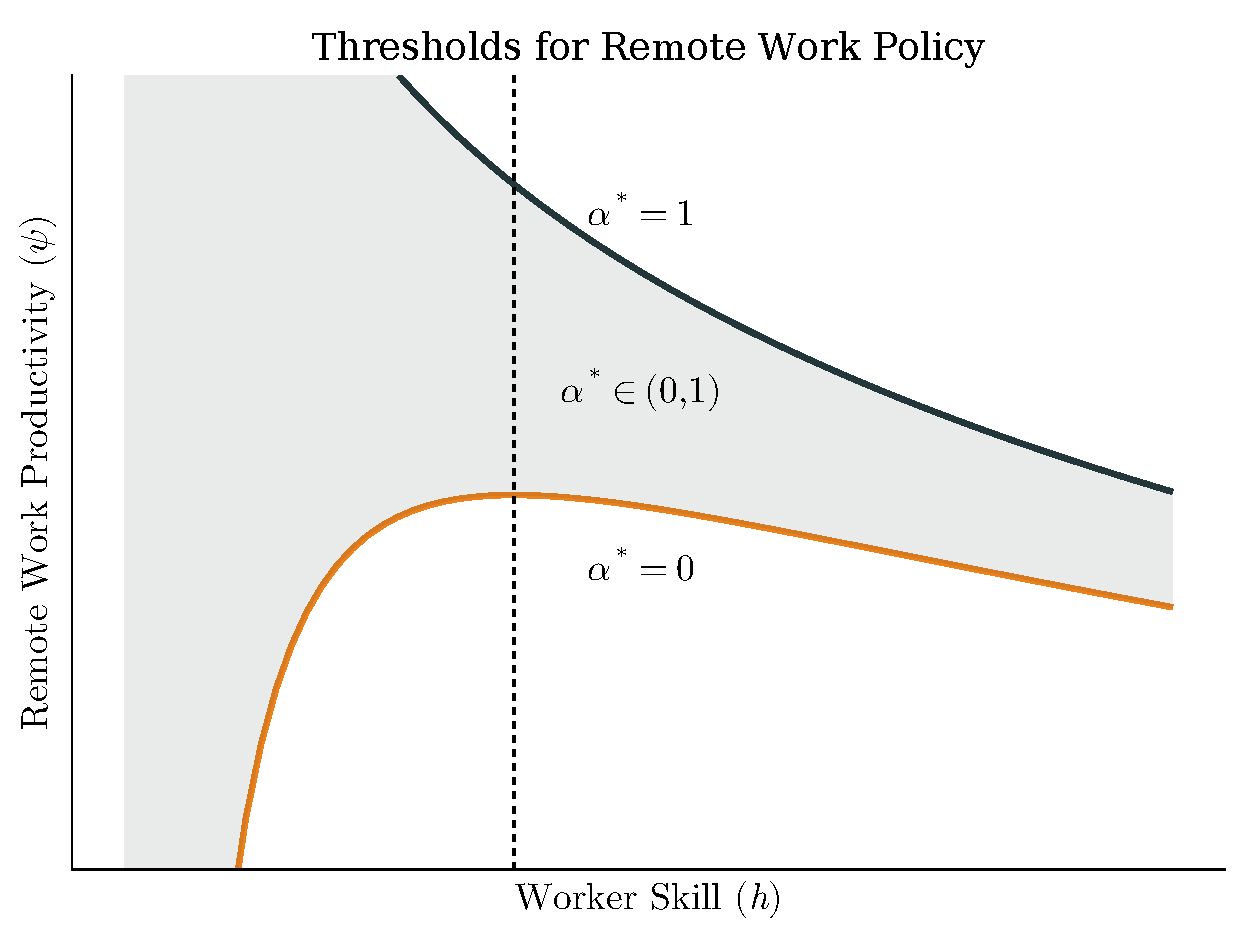
\includegraphics[width=0.65\linewidth,height=\textheight,keepaspectratio]{index_files/mediabag/plot_thresholds.pdf}

}

\caption{\label{fig-elephant}Lower \((\underline{\psi}(h))\) and upper
\(\overline{\psi}(h)\) thresholds variation with worker skill.}

\end{figure}%

Figure~\ref{fig-elephant} provides a graphical representation of the
thresholds for a parametrization with \(A_{0} = 0\). The declining
curves of \(\underline{\psi}(h)\) and \(\overline{\psi}(h)\) with higher
worker skill indicate that, as employees become more skilled, firms are
more likely to adopt remote work policies even when their efficiency
levels are moderate. This further underscores the importance of skill in
determining the mix of remote versus in-person work.

\begin{figure}

\centering{

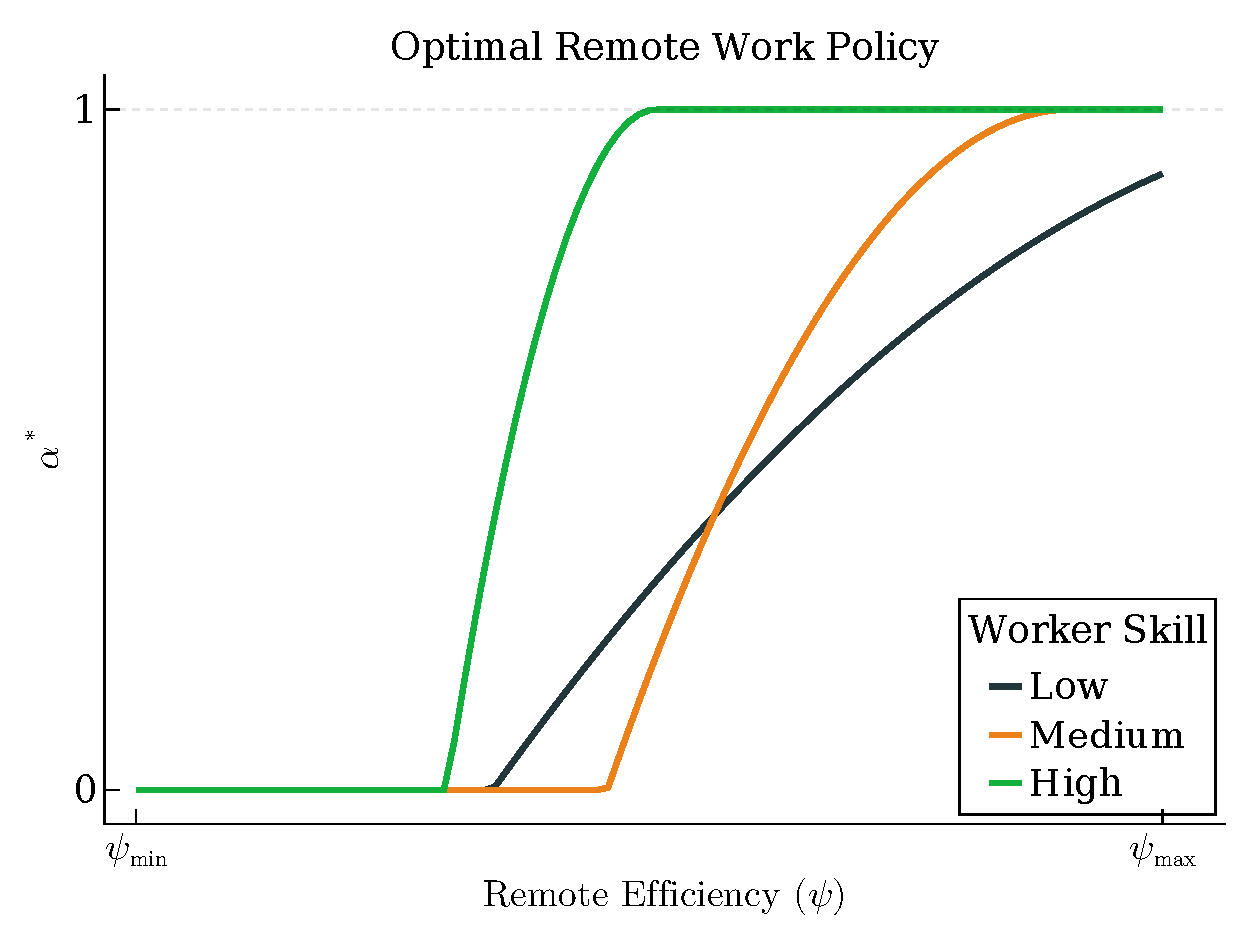
\includegraphics[width=0.65\linewidth,height=\textheight,keepaspectratio]{index_files/mediabag/plot_policy_for_skil.pdf}

}

\caption{\label{fig-el}Optimal remote work share \((\alpha^{*})\) for
different remote efficiency and skill levels.}

\end{figure}%

Figure~\ref{fig-el}, shows the optimal remote work share \(\alpha^*\) as
a function of firm remote work efficiency \(\psi\) across different
worker skill levels \(h\). The graph delineates regions where the
optimal \(\alpha^*\) takes on the values 0 (in-person work), between 0
and 1 (partial remote work), and 1 (full remote work). Notably, higher
worker skill shifts the transition thresholds, implying that more
skilled workers require lower firm efficiency to justify a shift towards
remote work. The chosen parametrization guarantees that the interior
solution \(\alpha^*(h)\) increases with \(h\).

\subsection{Labor Market Search}\label{sec-labor-market-search}

Both firms and workers discount the future at rate \(\beta\). Workers
are characterized by their type \(h\) and direct their search toward
submarkets distinguished by the promised utility level \(x\). A worker
of type \(h\) evaluates the different utility promises available in each
submarket and chooses to search in the one that maximizes their expected
value. This expected value incorporates not only the probability of
being hired but also the future discounted value of the job. At the same
time, firms target workers of a particular type \(h\) by posting job
offers (or contracts) that promise a specific utility level \(x\). This
setup allows the market to be segmented into different submarkets. The
tightness of a submarket \((h, x)\) is defined as:
\[ \theta(h, x) = \frac{v(h, x)}{u(h, x)}, \] where \(v(h, x)\) denotes
the number of vacancies posted by firms in the submarket and \(u(h, x)\)
represents the number of unemployed workers actively searching within
that particular submarket. This measure of tightness directly influences
the probabilities of matching: the vacancy filling rate
\(q(\theta(h, x))\) and the job finding rate \(p(\theta(h, x))\) are
both functions of \(\theta\). Matches are exogenously broken at a rate
\(\delta\). Free entry of firms, incurring a cost \(\kappa(x)\) per
vacancy posted (which may depend on the offered utility \(x\)), ensures
that market opportunities yielding positive expected profits are
exploited.

Once a firm and a worker are matched, the firm delivers the promised
utility \(x\) to the worker by applying the firm's optimal remote work
policy \(\alpha^*(\psi, h, x)\). Crucially, firms know their remote-work
efficiency parameter \(\psi\) \emph{before} deciding where to post
vacancies. The distribution of firm types in the overall economy is
given by \(F(\psi)\), which is common knowledge.

\textbf{Firm Value Functions and Probabilistic Choice:}

Firms choose strategically which submarket \((h, x)\) to target based on
the potential profitability of the match. The value of an ongoing match
for a firm of type \(\psi\) with a worker of type \(h\) under contract
\(x\), denoted \(J(\psi, h, x)\), is determined by the current payoff
plus the discounted expected continuation value:
\begin{equation}\phantomsection\label{eq-valueFirmMatch}{ J(\psi, h, x) = Y(\alpha^*(\psi, h, x) | \psi, h) - w(x, \alpha^*(\psi, h, x)) + \beta[(1 - \delta)J(\psi, h, x) + \delta V(\psi, h)], }\end{equation}
where \(V(\psi, h)\) represents the expected value for a firm of type
\(\psi\) upon returning to the market after separation. This value
reflects the optimal posting strategy, considering the expected returns
from different submarkets.

For a given worker type \(h\) and observed market vacancy filling rates
\(\{q(h, x')\}_{x'}\), a firm \(\psi\) evaluates the expected profit
from posting in each submarket \(x'\):
\[ \Pi_{post}(\psi, h, x') = q(h, x') J(\psi, h, x') - \kappa(x'). \]
Instead of deterministically choosing only the submarket(s) yielding the
absolute maximum profit, we adopt a \textbf{probabilistic choice
framework} (akin to a random utility model). Firms choose submarket
\(x\) with a probability \(P(x | \psi, h)\) that is increasing in the
potential profit \(\Pi_{post}(\psi, h, x)\). A common specification
(logit choice, derived from Type I Extreme Value shocks) gives:
\begin{equation}\phantomsection\label{eq-softmaxChoice}{ P(x | \psi, h) = \frac{\exp(\xi \cdot \Pi_{post}(\psi, h, x))}{\sum_{x''} \exp(\xi \cdot \Pi_{post}(\psi, h, x''))}, }\end{equation}
where \(\xi \ge 0\) is a parameter governing the sensitivity of choices
to profit differences. As \(\xi \to \infty\), the choice becomes
deterministic (only the maximum profit option is chosen); as
\(\xi \to 0\), choices become random across profitable options. Firms
only participate (i.e., \(P(x | \psi, h) > 0\) for some \(x\)) if the
maximum potential profit \(\max_{x'} \Pi_{post}(\psi, h, x')\) is
non-negative.

This probabilistic choice leads to \textbf{endogenous sorting} where
firms with characteristics \((\psi, h)\) that yield higher profits in
certain submarkets \(x\) are more likely to post vacancies there.

\textbf{Equilibrium and Free Entry:} In equilibrium, firms' expectations
about vacancy filling rates \(q(h,x)\) are consistent with the rates
generated by the market tightness \(\theta(h,x)\) resulting from firm
and worker decisions. Free entry ensures that, in active markets,
expected profits are driven down. Specifically, the equilibrium vacancy
filling rate \(q(h, x)\) adjusts such that the \emph{expected} profit
for a firm entering market \((h, x)\) is zero on average, considering
the mix of firms likely to choose that market. This implies:
\begin{equation}\phantomsection\label{eq-tightnessDeterminationSoftmax}{ q(h, x) \mathbb{E}\left[ J(\psi, h, x) \,|\, \text{firm } \psi \text{ chooses } (h,x) \right] = \kappa(x). }\end{equation}
The conditional expectation is calculated based on the choice
probabilities and the underlying firm distribution:
\begin{equation}\phantomsection\label{eq-conditionalJSoftmax}{ \mathbb{E}\left[ J(\psi, h, x) \,|\, \text{firm } \psi \text{ chooses } (h,x) \right] = \frac{\sum_{\psi'} J(\psi', h, x) P(x | \psi', h) f(\psi')}{\sum_{\psi''} P(x | \psi'', h) f(\psi'')}, }\end{equation}
where the denominator represents the total probability mass of firms
choosing market \((h,x)\). A market \((h,x)\) is active only if this
expected value is sufficient to cover the cost \(\kappa(x)\) (i.e.,
\(\mathbb{E}[J|h,x] > \kappa(x)\)). Infra-marginal firms (those with
high \(J(\psi, h, x)\) relative to the average) may still perceive a
positive expected profit from participating.

The distribution of firms encountered by workers searching in submarket
\((h, x)\) is the \emph{conditional distribution}, reflecting the
probabilistic choices. The conditional probability density function
(PDF) is:
\begin{equation}\phantomsection\label{eq-firmDensitySubmarketSoftmax}{ f(\psi \mid h, x) = \frac{P(x | \psi, h) f(\psi)}{\sum_{\psi'} P(x | \psi', h) f(\psi')} }\end{equation}
where the denominator is the total mass choosing \((h,x)\). The
conditional cumulative distribution function (CDF) \(F(\psi \mid h, x)\)
is obtained by integrating (or summing) this density:
\begin{equation}\phantomsection\label{eq-firmDistributionSubmarketSoftmax}{ F(\psi \mid h, x) = \int_{-\infty}^{\psi} f(\psi' \mid h, x) d\psi' = \frac{\sum_{\psi'' \le \psi} P(x | \psi'', h) f(\psi'')}{\sum_{\psi'} P(x | \psi', h) f(\psi')} }\end{equation}

\textbf{Worker Value Functions:} For workers, the value functions
capture the trade-off between being unemployed and employed. A worker of
type \(h\) chooses the submarket \(x\) that maximizes their expected
lifetime utility. The value of unemployment \(U(h)\) is:
\begin{equation}\phantomsection\label{eq-unemployedWorkerValue}{ U(h) = b + \beta \max_{x} \Biggl\{ p\bigl(\theta(h,x)\bigr) \mathbb{E}_{\psi|h,x} \left[ W(\psi, h, x) \right] + \Bigl(1 - p\bigl(\theta(h,x)\bigr)\Bigr) U(h)\Biggr\}, }\end{equation}
where \(p(\theta(h, x))\) is the job finding rate, and the expectation
\(\mathbb{E}_{\psi|h,x}[\cdot]\) uses the conditional distribution
\(F(\psi | h, x)\) from
Equation~\ref{eq-firmDistributionSubmarketSoftmax}:
\[ \mathbb{E}_{\psi|h,x} \left[ W(\psi, h, x) \right] = \int W(\psi', h, x) \, dF(\psi' | h, x) = \sum_{\psi'} W(\psi', h, x) f(\psi' | h, x). \]
This reflects that workers anticipate the specific mix of firms
attracted to each submarket \((h, x)\).

Once employed with a firm of type \(\psi\) under contract \(x\), the
worker's value \(W(\psi, h, x)\) evolves according to:
\begin{equation}\phantomsection\label{eq-employedWorkerValue}{ W(\psi, h, x) = x + \beta\Bigl[(1-\delta)W(\psi, h, x) + \delta\,U(h)\Bigr]. }\end{equation}

The equilibrium vacancy filling rates \(q^*(h, x)\), market tightnesses
\(\theta^*(h, x)\), firm choice probabilities \(P^*(x | \psi, h)\), and
the resulting conditional distribution of firms \(f^*(\psi | h, x)\) are
determined simultaneously. These objects satisfy the firm's
probabilistic choice rule Equation~\ref{eq-softmaxChoice}, the free
entry condition Equation~\ref{eq-tightnessDeterminationSoftmax} based on
the conditional expectation Equation~\ref{eq-conditionalJSoftmax}, and
consistency with the underlying matching technology \(q(\theta)\). We
solve for this equilibrium numerically using an iterative algorithm
detailed in Appendix~\ref{sec-appendix-endogenousFirmDistribution}.

\section{Calibration}\label{calibration}

This section details the procedure used to discipline the model and
obtain plausible values for key structural parameters governing firm
production, worker skills, and firm efficiency distributions. Our
approach combines econometric estimation using detailed
industry-occupation data with calibration techniques to map estimated
coefficients to the model's parameters. We leverage data from the Bureau
of Labor Statistics (OES, Productivity), the American Community Survey
(ACS), the Census Bureau's Business Dynamics Statistics (BDS), and the
O*NET database.

\subsection{Data Sources and Variable
Construction}\label{data-sources-and-variable-construction}

We construct a panel dataset primarily at the 3-digit NAICS industry
level, spanning the period form 2013 to 2023 . Key variables include:

\begin{itemize}
\tightlist
\item
  \textbf{Output per Hour:} Derived from BLS sectoral productivity data,
  adjusted for price deflation. This serves as our measure of \(Y/L\) in
  the data.
\item
  \textbf{Industry Skill Index:} Constructed by weighting
  occupation-level skill indices derived from O*NET data (combining
  normalized importance and level ratings for relevant skills and
  abilities) by their employment shares within each industry, using BLS
  OES data. This proxies for the average \(h\) within an industry.
\item
  \textbf{Industry Teleworkability Index:} Self-constructed index based
  on the Teleworkability Index at the occupation level. The procedure is
  described in the next section, weighted by employment shares within
  industries.
\item
  \textbf{Observe Remote Work Rates:} Measured using data from the ACS,
  representing the observed share of remote work in each industry-year.
\end{itemize}

\subsection{Estimating the Occupation Teleworkability
Index}\label{sec-teleworkability}

A key input into our structural model is the heterogeneity in firms'
remote work efficiency (\(\psi\)). We require an empirical counterpart
to discipline the distribution of this parameter. Existing indices of
occupation-level remote work feasibility, such as the binary
classification by (Dingel and Neiman 2020) or the index by (Mongey,
Pilossoph, and Weinberg 2020), provide valuable benchmarks. These
approaches typically involve selecting key occupational characteristics
based on theoretical considerations or researcher assessment to
determine teleworkability. To leverage a richer, data-driven approach
using a high-dimensional feature set, we construct a novel
\textbf{Teleworkability Index} using machine learning techniques on
detailed occupational data. This index aims to capture both whether an
occupation \emph{can} be performed remotely (extensive margin) and the
\emph{degree} to which it is feasible (intensive margin).

\textbf{Data:} Our primary feature set consists of detailed
occupation-level characteristics from the O*NET database, encompassing a
wide range of variables related to skills, abilities, work activities,
and work context. For supervised learning, we utilize data from the
Occupational Requirements Survey, which reports the share of workers in
each occupation for whom telework is available. In 2024, telework was
available to 14.9\% of civilian workers. We normalize this variable to a
{[}0, 1{]} scale. As ORS coverage is incomplete, this provides labels
for a subset of occupations.

\textbf{Methodology:} We employ a two-stage modeling approach using
Random Forest models, leveraging their ability to handle
high-dimensional data and capture non-linear relationships. Both models'
hyperparameters are tuned using cross-validation techniques on the
training data.

\begin{enumerate}
\def\labelenumi{\arabic{enumi}.}
\item
  \textbf{Stage 1: Classification (Extensive Margin):} We first train a
  \emph{Random Forest Classifier} to distinguish occupations where
  telework is impossible (ORS label = 0) from those where it is at least
  partially possible (ORS label \textgreater{} 0). The model is trained
  on the labeled subset of occupations using the binary indicator
  derived from the ORS label. This stage identifies occupations
  fundamentally unsuited for remote work, which is particularly
  important because of the large amounts of zeros in the training data.
\item
  \textbf{Stage 2: Regression (Intensive Margin):} For occupations
  identified as having \emph{non-zero} teleworkability by the ORS
  labels, we train a \emph{Random Forest Regressor}. To ensure
  predictions remain within the {[}0, 1{]} bound and to better handle
  the distribution of the target variable, we apply a logit
  transformation (\(\log(y / (1-y))\)) to the non-zero ORS labels before
  training. The regressor learns the relationship between ONET features
  and the \emph{degree} of teleworkability for jobs where remote work is
  feasible.
\end{enumerate}

\begin{figure}

\centering{

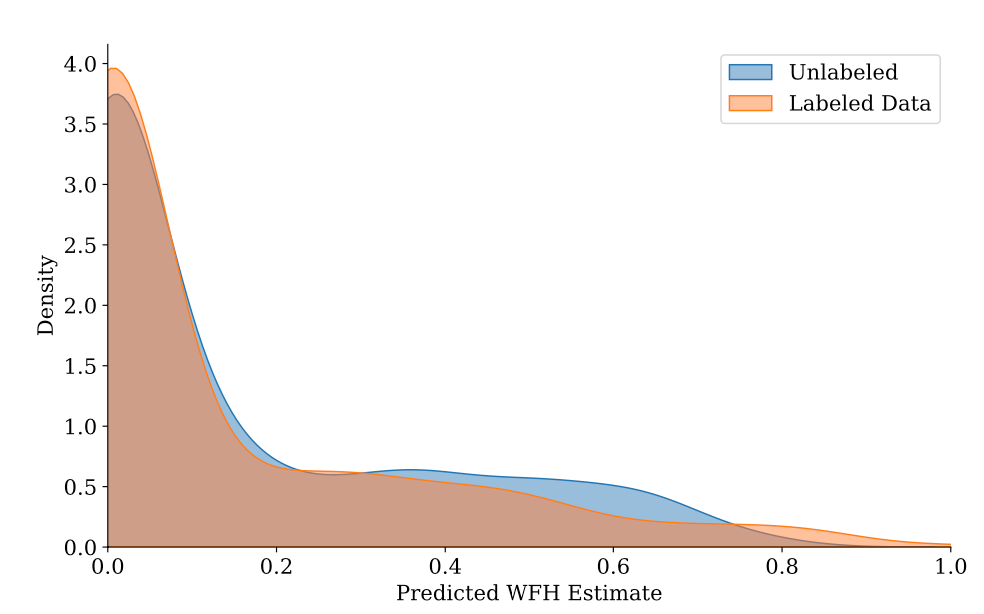
\includegraphics[width=0.85\linewidth,height=\textheight,keepaspectratio]{index_files/mediabag/SCR-20250417-t92.png}

}

\caption{\label{fig-dist_labeled_unlabeled}}

\end{figure}%

\textbf{Validation and Prediction:} The performance of the tuned
two-stage model is evaluated using bootstrap validation on held-out test
data, assessing metrics such as Accuracy and F1-score for the
classifier, and Mean Squared Error (MSE) and Correlation for the
regressor . The classifier achieved an accuracy of 90.7\% along with an
F1 score of 91.9\%, while the regression model recorded a mean squared
error (MSE) of 0.1 and a correlation of 0.71;
Figure~\ref{fig-dist_labeled_unlabeled} shows the distribution of
predicted teleworkability indices for both labeled and unlabeled data.
The final trained model is then used to predict the teleworkability
index for \emph{all} occupations in the O*NET database, including those
without ORS labels. For a given occupation:

\begin{itemize}
\tightlist
\item
  The classifier predicts the probability of it being a
  zero-teleworkability job. If this probability exceeds a threshold, the
  index is set to 0.
\item
  Otherwise, the regressor predicts the logit-transformed level of
  teleworkability, which is then converted back to the {[}0, 1{]} scale
  using the inverse logit function.
\end{itemize}

This resulting continuous index represents our measure of
occupation-level teleworkability.

\textbf{Linking to the Model:} This estimated occupation-level
Teleworkability Index forms the basis for constructing our
industry-level \(\text{TELE}\) variable (by weighting occupational
indices by employment shares within industries). Furthermore, the
relationship estimated that we estimate allows us to use the
distribution of this index across industries (weighted by firm creation)
to empirically inform the aggregate distribution of firm remote work
efficiency, \(F(\psi)\), that we supply externally to the structural
model.

\subsection{Estimation of Production Function
Components}\label{estimation-of-production-function-components}

To inform the parameters of the model's production function,
\(Y = A(h) ((1-\alpha) + \alpha g(\psi, h))\), we estimate a
reduced-form relationship between productivity, skills, remote work, and
teleworkability using our panel data. We assume that the industry-level
data reflects the aggregate outcomes of the firm-level production
specified in the model. Specifically, we relate the firm's remote work
efficiency \(g(\psi, h)\) to the observed industry teleworkability
(\(\text{TELE}\)) and potentially worker skill (\(\text{SKILL}\)), and
the baseline productivity \(A(h)\) to worker skill (\(\text{SKILL}\)).

Our preferred specification is:\\
\begin{equation}\label{eq:reducedFormProd}
\begin{aligned}
    \log(\text{OUTPUT}_{it}) ={}& \beta_0 \cdot \text{SKILL}_{it} \\
    & + \beta_1 \cdot (\text{ALPHA}_{it} \times \text{SKILL}_{it}) \\
    & + \beta_2 \cdot (\text{TELE}_{it} \times \text{ALPHA}_{it} \times \text{SKILL}_{it}) \\
    & + \beta_3 \cdot (\text{SKILL}_{it} \times \log(\text{SKILL}_{it})) \\
    & + \mu_i + \lambda_t + \epsilon_{it}
\end{aligned}
\end{equation}

where \(i\) denotes industry and \(t\)~denotes year,~\(\mu_{i}\)~are
sector fixed effects, and~\(\lambda_{t}\)~are year fixed effects. The
regression results are summarized in Table 4.

\begin{table}[h]  
\centering  
\fontsize{8}{10}\selectfont  
\begin{tabular}{lrrrrr}
\toprule
                                   &                   \multicolumn{5}{c}{OUTPUT}                   \\ 
\cmidrule(lr){2-6} 
                                   &        (1) &        (2) &        (3) &        (4) &        (5) \\ 
\midrule
(Intercept)                        &   16.739** &            &            &            &            \\ 
                                   &    (6.424) &            &            &            &            \\ 
SKILL                              &  25.708*** &  23.910*** &  26.279*** &  37.024*** &  39.948*** \\ 
                                   &    (2.353) &    (2.266) &    (2.495) &    (2.922) &    (3.158) \\ 
ALPHA $\times$ SKILL               &   -37.564* &   -34.714* &   -53.873* &    -29.745 &  -84.807** \\ 
                                   &   (15.298) &   (15.366) &   (26.421) &   (15.311) &   (26.700) \\ 
SKILL $\times$ log(SKILL)          &  64.152*** &  15.974*** &  63.632*** & 149.791*** & 157.405*** \\ 
                                   &   (18.611) &    (2.148) &   (18.837) &   (22.199) &   (22.526) \\ 
TELE $\times$ ALPHA $\times$ SKILL & 315.199*** & 286.139*** & 356.831*** &   176.199* &  318.733** \\ 
                                   &   (70.115) &   (69.705) &   (89.545) &   (78.090) &   (96.738) \\ 
\midrule
YEAR Fixed Effects                 &            &            &        Yes &            &        Yes \\ 
SECTOR Fixed Effects               &            &            &            &        Yes &        Yes \\ 
\midrule
$N$                                &        418 &        418 &        418 &        418 &        418 \\ 
$R^2$                              &      0.263 &      0.510 &      0.265 &      0.378 &      0.388 \\ 
Within-$R^2$                       &            &            &      0.264 &      0.292 &      0.303 \\ 
\bottomrule
\end{tabular} 
\caption{Regression results for industry-level output estimation}  
  
\end{table}

\begin{table}
\centering
\begin{tabular}{lcc}
\hline
\textbf{Parameter} & \textbf{Mapping} & \textbf{Value} \\
\hline
$A$ & $\beta_0$ & 25.71 \\
$\psi_0$ & $(\beta_1 + 1) / A$ & -1.42 \\
$\psi_{1}$ & $\beta_2 / A$ & 12.26 \\
$\phi$ & $\beta_3 / A$ & 2.50 \\
$C$ & \text{(Intercept)} & 16.74 \\
\hline
\end{tabular}
\caption{Model Parameters, Mappings to Regression Coefficients, and Values}

\end{table}

\textbf{Mapping Estimates to Structural Parameters}

We map the estimated coefficients from \eqref{eq:reducedFormProd}
(specifically, using the results from model \((1)\)) to the parameters
of our assumed functional forms for \(A(h)\) and \(g(\psi, h)\). with
the parametric assumption
\[Y = A(h) (1 + \alpha (g(\psi, h) - 1))\qquad \text{with} \quad g(\psi, h) \approx \psi_0 + \psi + \phi \log h \:\text{ and }\: A(h)=A_{1} h\]

We derive the structural parameters \(A_1, \phi, \psi_0, \psi_1\) The
estimated values used in the model simulation are presented in Table 5.

\textbf{Estimating Distributions}

\begin{figure}

\centering{

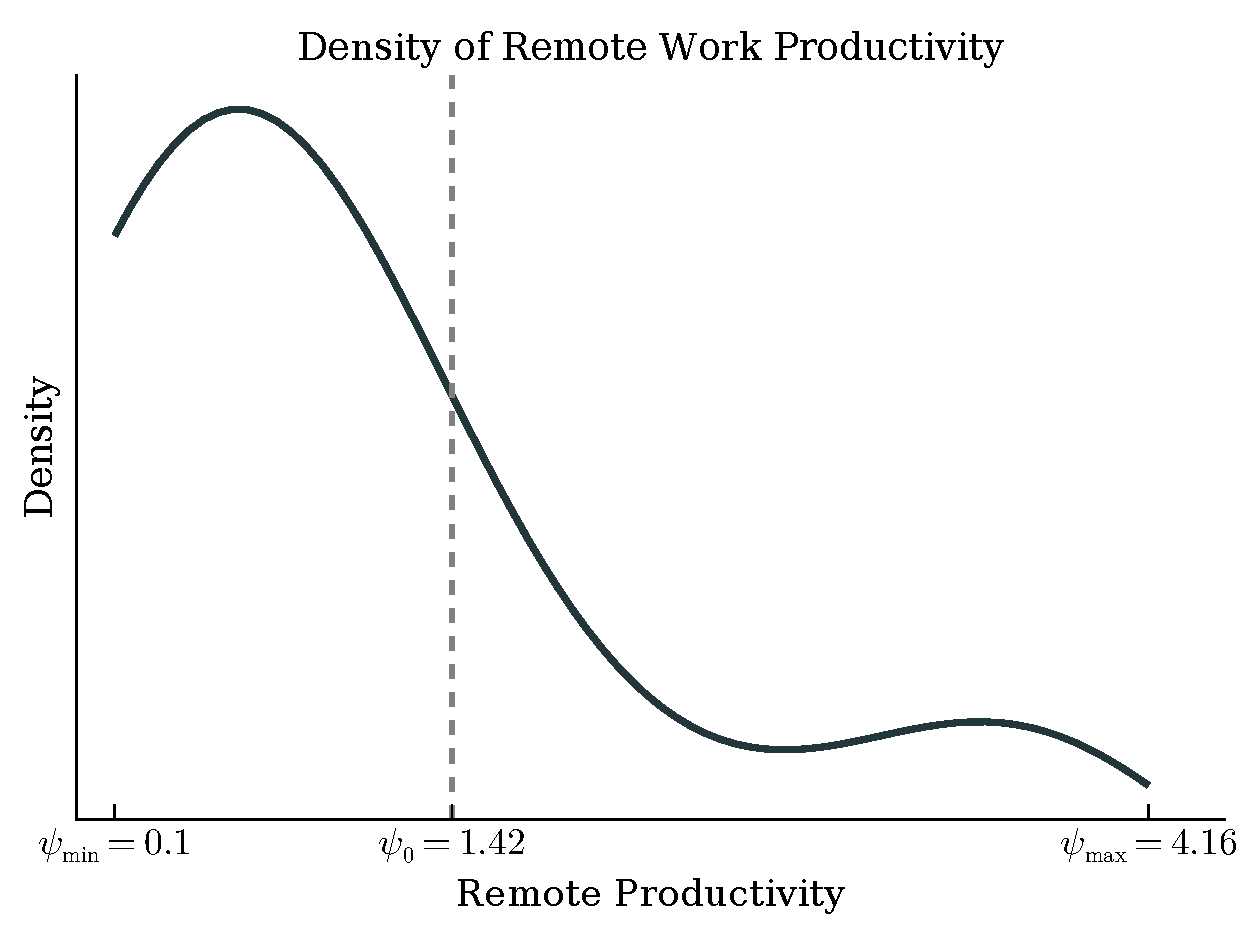
\includegraphics[width=0.5\linewidth,height=\textheight,keepaspectratio]{index_files/mediabag/productivity_density.pdf}

}

\caption{\label{fig-remote-productivity-density}}

\end{figure}%

\begin{itemize}
\tightlist
\item
  \textbf{Firm Type Distribution \(F(\psi)\):} We use the relationship
  derived from the regression,
  \(\psi \approx \psi_1 \times \text{TELE}_{i}\), to obtain an estimate
  of the average firm type \(\psi_i\) for each industry \(i\). Using
  industry weights based on job creation from new firms (from BDS), we
  estimate the aggregate distribution of firm types \(f(\psi)\) using
  Kernel Density Estimation (KDE). The resulting distribution
  Figure~\ref{fig-remote-productivity-density} captures the
  heterogeneity in remote work efficiency across the economy. We then
  discretize this distribution onto the model's \(\psi_{grid}\).
\end{itemize}

\begin{figure}

\centering{

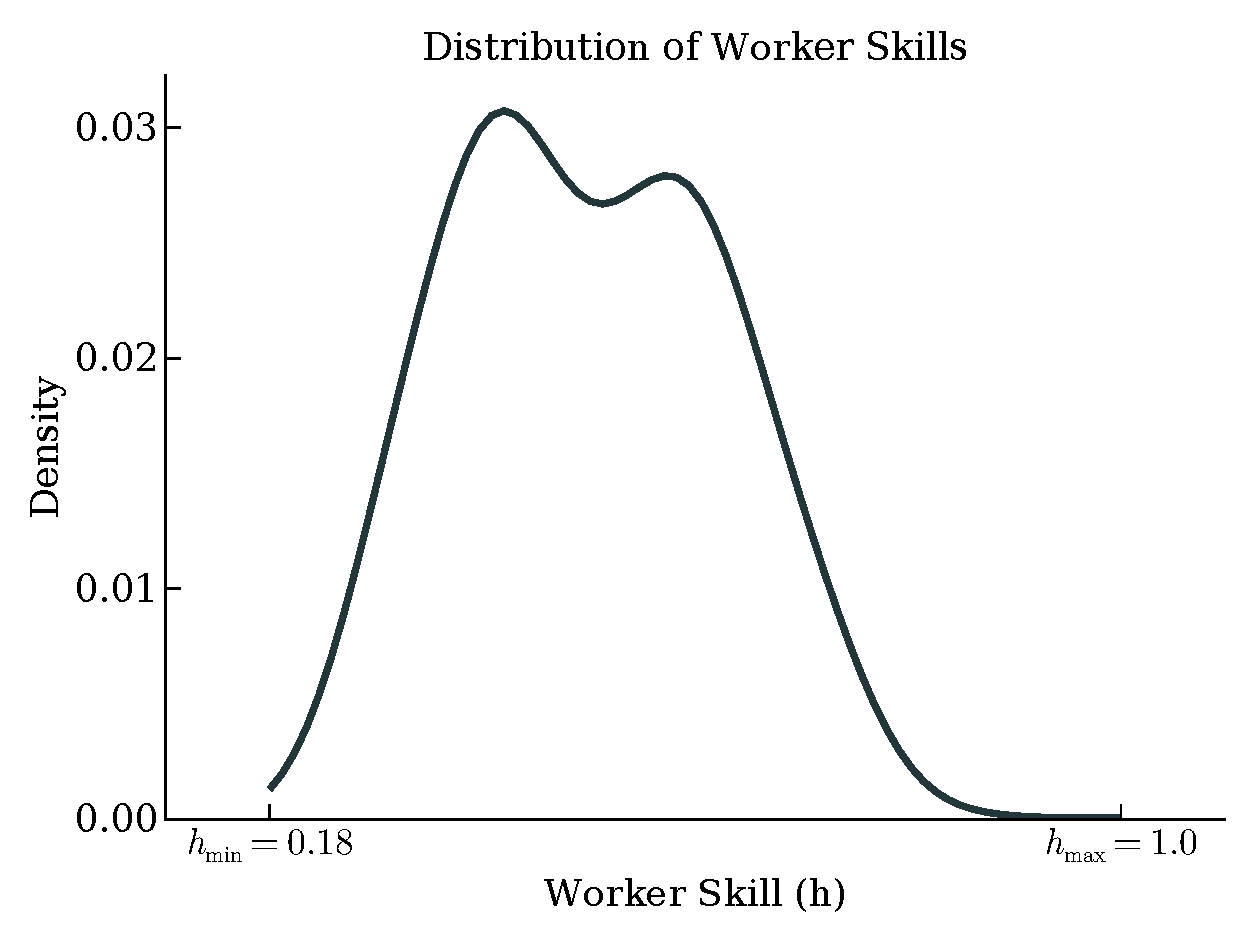
\includegraphics[width=0.5\linewidth,height=\textheight,keepaspectratio]{index_files/mediabag/worker_type_distribu.pdf}

}

\caption{\label{fig-skill-density}}

\end{figure}%

\begin{itemize}
\tightlist
\item
  \textbf{Worker Skill Distribution \(F(h)\):} We construct the
  aggregate distribution of worker skills \(f(h)\) similarly. We use the
  occupation-level skill indices derived from O*NET and weight them by
  their aggregate employment. We then fit a KDE to these weighted skill
  indices to obtain the distribution \(f(h)\)
  Figure~\ref{fig-skill-density} and discretize it onto the model's
  \(h_{grid}\).
\end{itemize}

\textbf{Calibration of Remaining Parameters} Several model parameters
are not directly identified by the estimation procedure above and are
calibrated using standard values from the literature or set to match
specific aggregate targets.

\begin{itemize}
\tightlist
\item
  \textbf{Discount Factor (\(\beta\)):} Set to \(0.9615\) corresponding
  to an annual discount rate of 4\%.
\item
  \textbf{Exogenous Separation Rate (\(\delta\)):} Set to \(0.07\).
\item
  \textbf{Matching Function Exponent (\(\gamma\)):} Set to \(0.6\)
  following (Menzio and Shi 2010)
\item
  \textbf{Unemployment Benefit (\(b\)):} Set the unemployment benefit as
  \(0.6\) of the potential wage the~lowest skill worker
\end{itemize}

\section{Results}\label{results}

This section presents the key qualitative predictions generated by
simulating our directed search model, using the parameters and
distributions estimated and calibrated as detailed in Section 4. We
focus on how the interplay between worker skill (\(h\)), firm remote
work efficiency (\(\psi\)), utility-dependent posting costs
(\(\kappa(x)\)), and probabilistic firm choices shapes labor market
outcomes.

\begin{figure}

\centering{

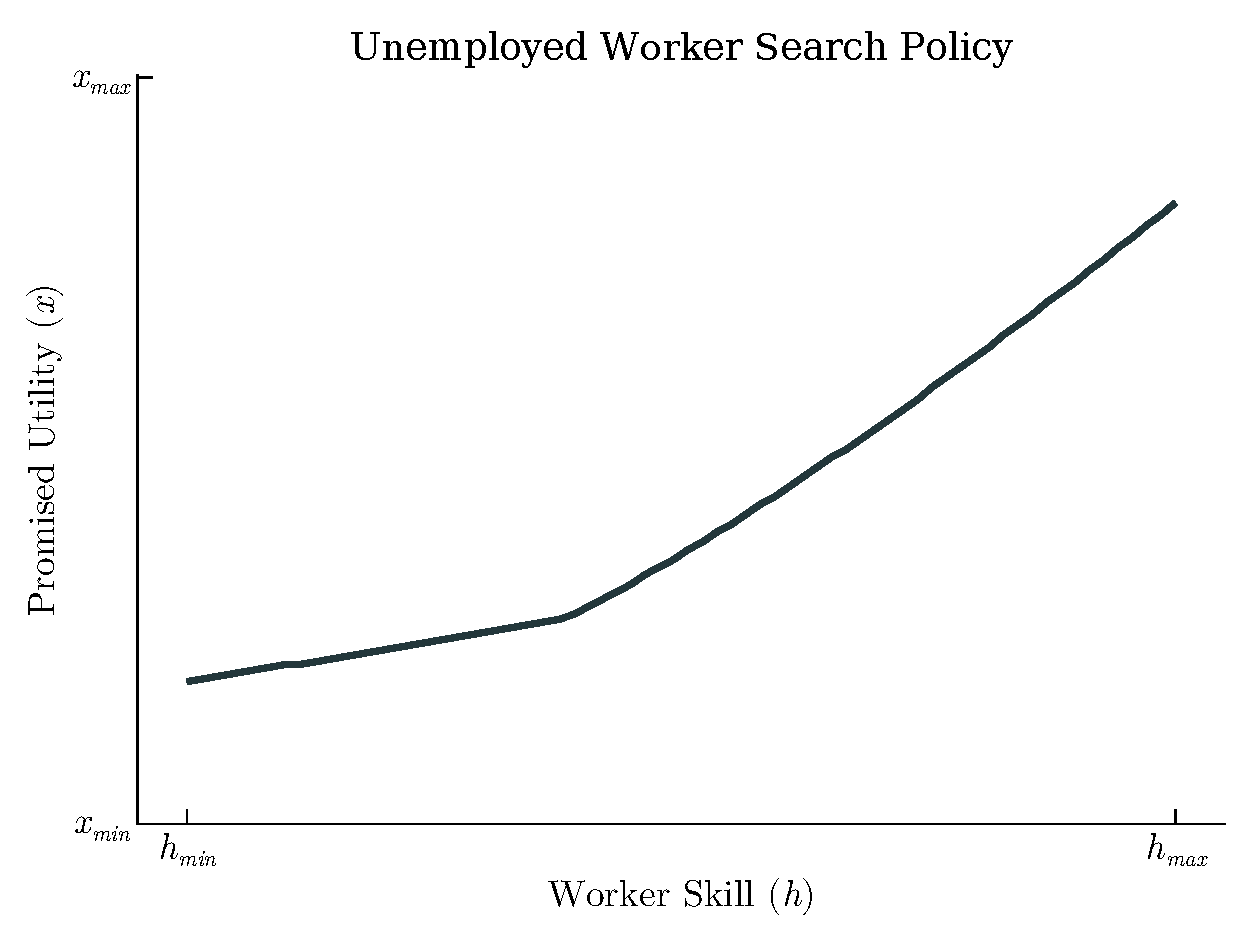
\includegraphics[width=0.6\linewidth,height=\textheight,keepaspectratio]{index_files/mediabag/worker_search_policy.pdf}

}

\caption{\label{fig-worker_search_policy}Higher skill workers target
higher utility submarkets.}

\end{figure}%

\textbf{Worker Search Behavior:} The model predicts workers' optimal
search strategies across utility submarkets. Figure
Figure~\ref{fig-worker_search_policy} plots the optimal promised utility
level \(x^*(h)\) targeted by workers of different skill levels \(h\).
Consistent with intuition, higher-skilled workers, who generate more
value in matches, direct their search towards submarkets offering higher
lifetime utility. This reflects their ability to command better
compensation packages, which include both wages and remote work
flexibility.

This confirms that the model generates sorting where more efficient
firms compete for more skilled workers by offering more attractive
utility packages.

\begin{figure}

\centering{

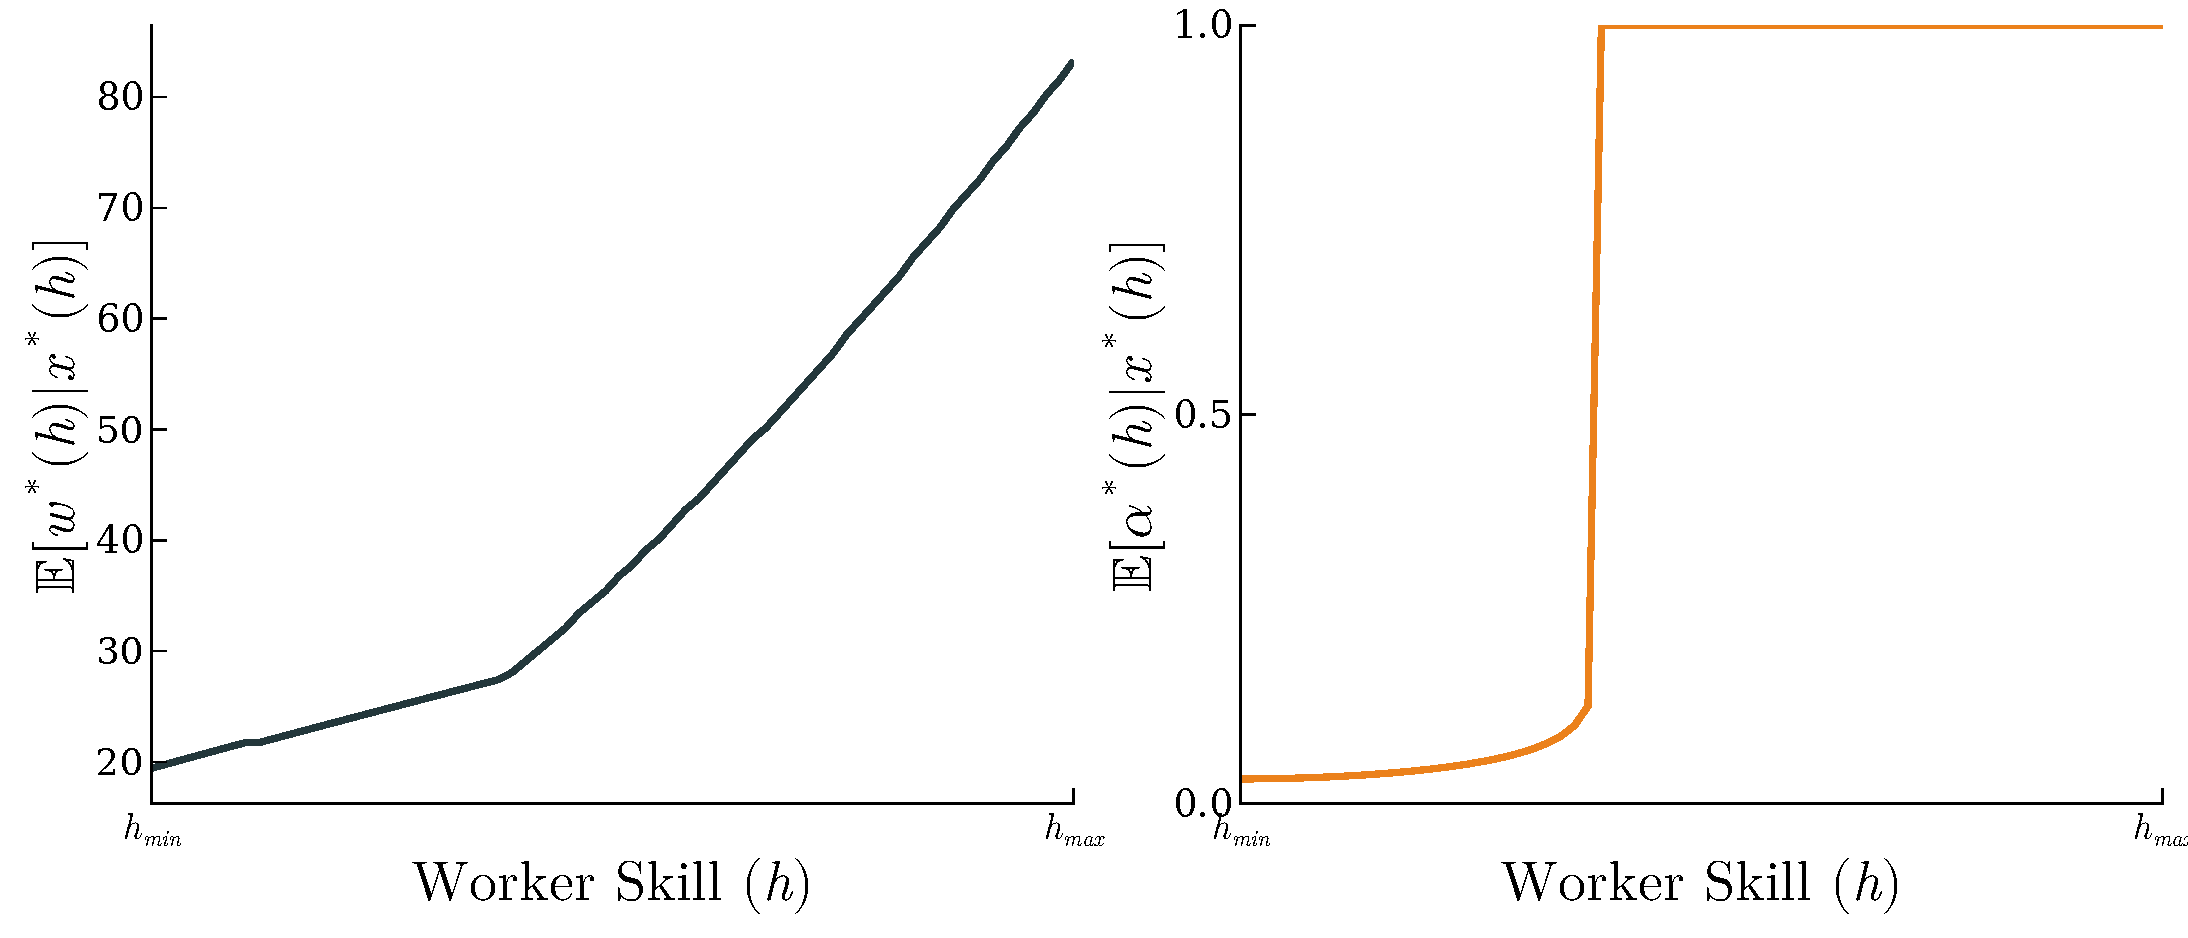
\includegraphics[width=0.8\linewidth,height=\textheight,keepaspectratio]{index_files/mediabag/wage_and_remote.pdf}

}

\caption{\label{fig-expected_outcomes}The model generates a positive
correlation of skill with both expected wage and expected remote work
share.}

\end{figure}%

\textbf{Expected Wages and Remote Work:} The sorting patterns translate
into equilibrium wage and remote work outcomes. Figure
Figure~\ref{fig-expected_outcomes} plots the expected wage
\(\mathbb{E}[w | h, x^*(h)]\) and expected remote work share
\(\mathbb{E}[\alpha^* | h, x^*(h)]\) for workers across the skill
distribution, calculated using the conditional distribution of firms
\(f^*(\psi | h, x^*(h))\) in their optimally chosen submarket
\(x^*(h)\). As expected, higher-skilled workers command significantly
higher wages. Furthermore, the expected share of remote work
\(\alpha^*\) also increases with worker skill \(h\). This arises because
higher-\(h\) workers sort into markets with higher-\(\psi\) firms, and
these firms, being more efficient at remote work, optimally offer a
greater share of remote time (\(\alpha^*\)) as part of the utility
package \(x^*(h)\).

\begin{figure}

\centering{

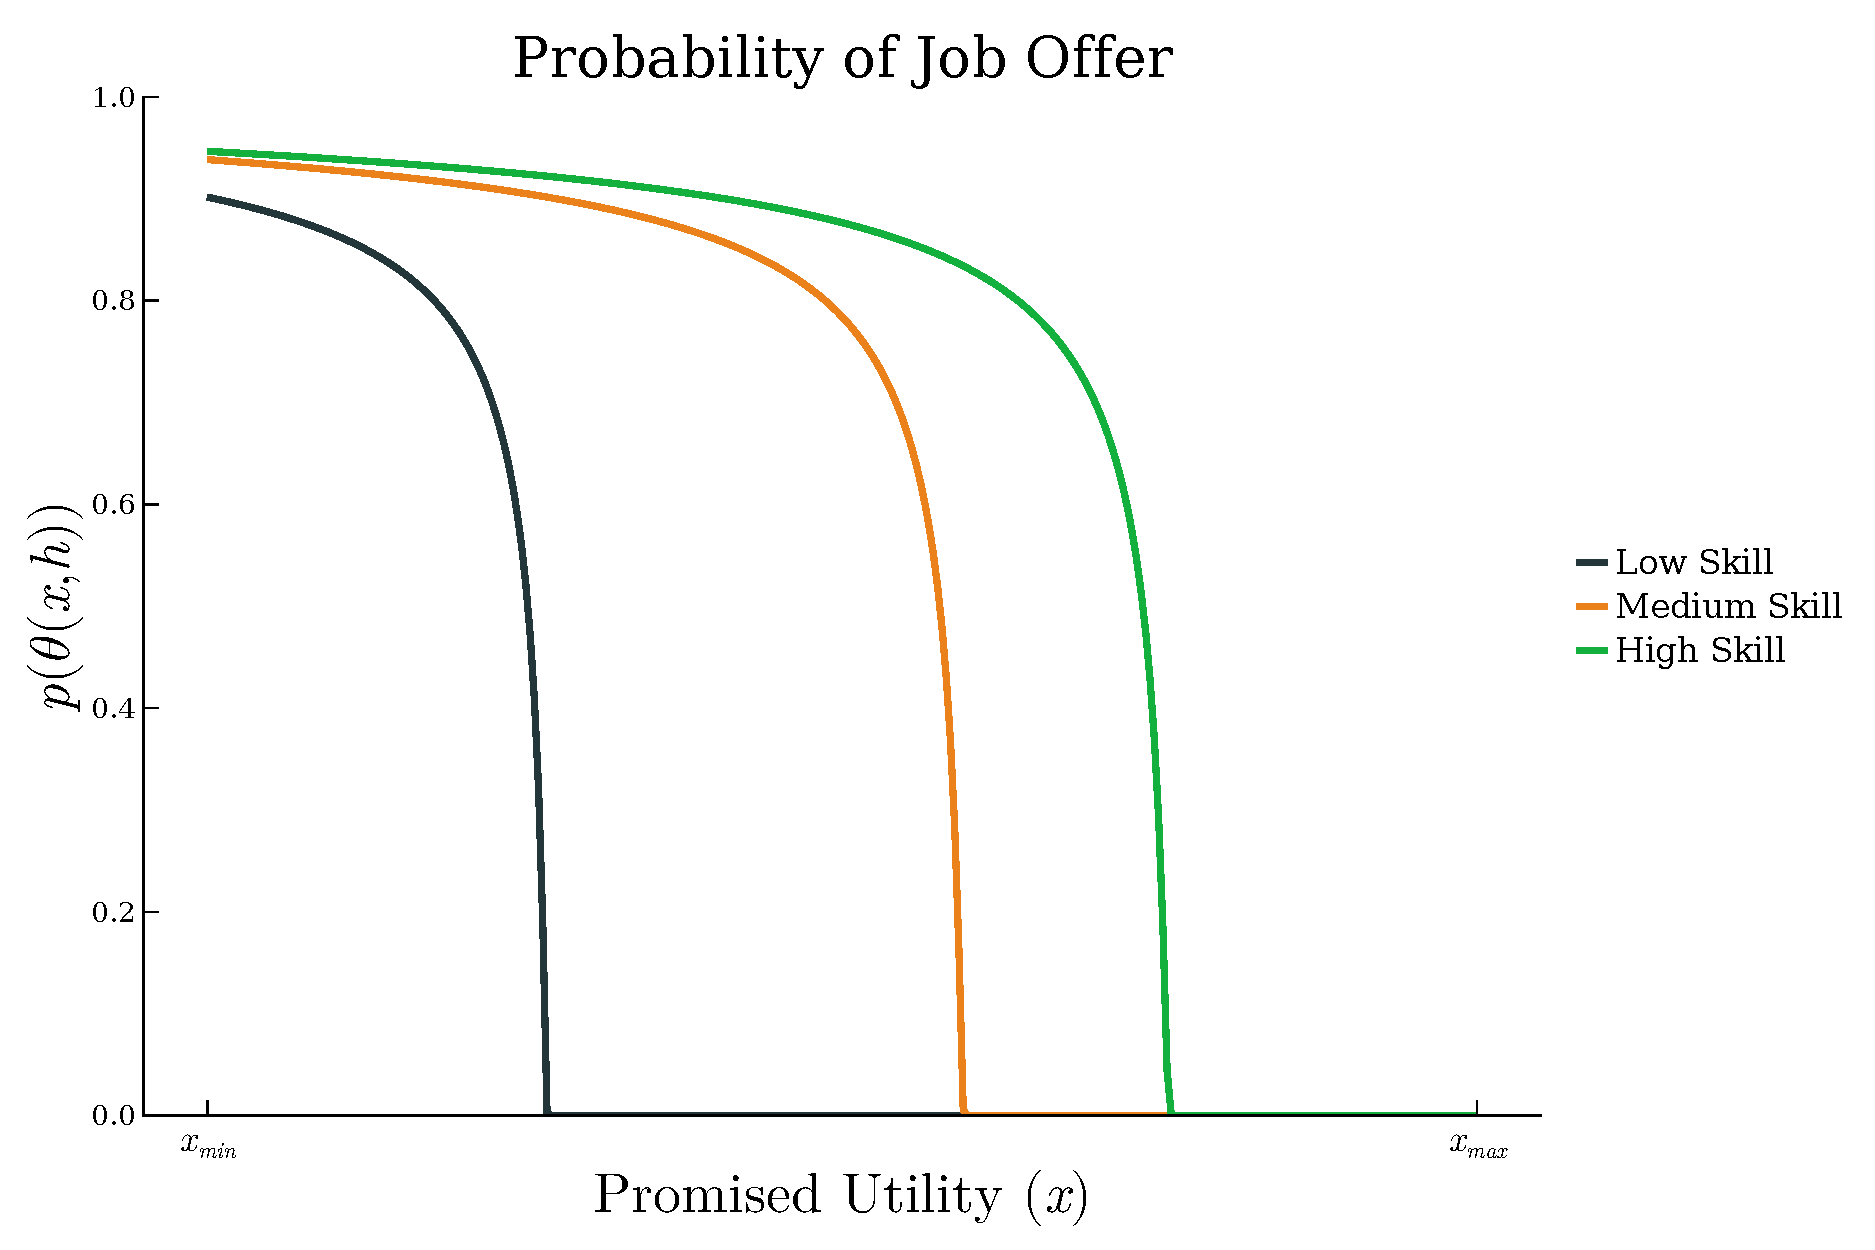
\includegraphics[width=0.8\linewidth,height=\textheight,keepaspectratio]{index_files/mediabag/job_finding_prob.pdf}

}

\caption{\label{fig-job_finding_prob}}

\end{figure}%

\textbf{Market Outcomes: Job Finding Rates:} Figure
Figure~\ref{fig-job_finding_prob} illustrates the equilibrium
job-finding probability \(p(\theta^*(h, x))\) faced by workers in
different submarkets. While multiple markets might be theoretically
available, workers concentrate their search in the market \(x^*(h)\)
offering the highest expected value. The plot shows
\(p(\theta^*(h, x))\) across the range of potential utility offers \(x\)
for representative low, medium, and high-skilled workers. We observe
that for each skill level, the job-finding probability decreases as the
offered utility \(x\) increases, reflecting the higher cost and
potentially lower equilibrium \(q^*\) in higher-utility markets.
However, higher-skilled workers can access markets with higher utility
levels before the job-finding probability drops to zero, consistent with
their higher market value.

\textbf{Summary of Results:} The simulated model, parameterized using
our empirical strategy, successfully generates key qualitative features
consistent with labor market observations. It produces positive
assortative matching between worker skill and firm efficiency, mediated
through directed search over utility offers. This sorting leads to
higher-skilled workers targeting and receiving higher utility offers,
which translates into higher expected wages and a greater expected share
of remote work. The model highlights how firm heterogeneity in remote
work efficiency and utility-dependent posting costs can shape
equilibrium wages and work arrangements.

\section{Conclusion}\label{conclusion}

This paper investigates the persistent wage premium observed for remote
workers in the United States. We begin by documenting key empirical
facts using ACS, O*NET, and BLS data: remote workers are positively
selected on earnings and education, occupations suitable for remote work
command higher wages, a significant WFH premium exists even within
detailed occupations, and this premium has evolved over time, increasing
notably since the COVID-19 pandemic. These findings motivate our central
question: what drives the wage gap between remote and non-remote
employees?

To explore potential mechanisms beyond observable characteristics, we
developed a directed search model featuring heterogeneity in worker
skill and firm remote work efficiency. In our framework, firms
strategically post utility offers (bundles of wages and remote work to
attract specific worker types, incurring utility-dependent posting
costs.

Workers direct their search towards utility offers that maximize their
expected value. Firms make probabilistic choices over which submarket to
enter, leading to endogenous sorting.

We estimate key production function parameters and distributions using
industry-level data and calibrate the remaining parameters. Simulating
the calibrated model reveals that it successfully generates positive
assortative matching: higher-skilled workers target and match with
higher-efficiency firms offering greater utility. Crucially, these
higher utility packages optimally bundle both higher wages and a greater
share of remote work for high-skill workers matched with high-efficiency
firms.

Our results provide a structural explanation for the WFH premium,
attributing it significantly to sorting dynamics and heterogeneity in
firms' ability to effectively implement remote work. The model
demonstrates how competition for high-skill workers leads efficient
firms to offer attractive packages where remote work acts partially as
an amenity but is also bundled with higher wages reflecting the value
generated in these high-productivity matches. The framework highlights
that understanding the WFH premium requires considering not just worker
preferences or average productivity effects, but also the equilibrium
sorting outcomes driven by firm-level heterogeneity in remote work
capabilities and the costs associated with different contract offers.
Future work could further explore the role of worker preferences and
dynamic considerations like on-the-job search.

\section*{References}\label{references}
\addcontentsline{toc}{section}{References}

\phantomsection\label{refs}
\begin{CSLReferences}{1}{0}
\bibitem[\citeproctext]{ref-barrero2023evolution}
Barrero, José Marı́a, Nicholas Bloom, and Steven J Davis. 2023. {``The
Evolution of Work from Home.''} \emph{Journal of Economic Perspectives}
37 (4): 23--49.

\bibitem[\citeproctext]{ref-bloom2015does}
Bloom, Nicholas, James Liang, John Roberts, and Zhichun Jenny Ying.
2015. {``Does Working from Home Work? Evidence from a Chinese
Experiment.''} \emph{The Quarterly Journal of Economics} 130 (1):
165--218.

\bibitem[\citeproctext]{ref-davis2021work}
Davis, Morris A, Andra C Ghent, and Jesse M Gregory. 2021. {``The
Work-from-Home Technology Boon and Its Consequences.''} National Bureau
of Economic Research.

\bibitem[\citeproctext]{ref-dingelHowManyJobs2020}
Dingel, Jonathan I., and Brent Neiman. 2020. {``How Many Jobs Can Be
Done at Home?''} \emph{Journal of Public Economics} 189 (September):
104235. \url{https://doi.org/10.1016/j.jpubeco.2020.104235}.

\bibitem[\citeproctext]{ref-gariety2007wage}
Gariety, Bonnie Sue, and Sherrill Shaffer. 2007. {``Wage Differentials
Associated with Working at Home.''} \emph{Monthly Lab. Rev.} 130: 61.

\bibitem[\citeproctext]{ref-holgersen2021and}
Holgersen, Henning, Zhiyang Jia, and Simen Svenkerud. 2021. {``Who and
How Many Can Work from Home? Evidence from Task Descriptions.''}
\emph{Journal for Labour Market Research} 55 (1): 1--13.

\bibitem[\citeproctext]{ref-mas2017valuing}
Mas, Alexandre, and Amanda Pallais. 2017. {``Valuing Alternative Work
Arrangements.''} \emph{American Economic Review} 107 (12): 3722--59.

\bibitem[\citeproctext]{ref-menzio2010a}
Menzio, Guido, and Shouyong Shi. 2010. {``Block Recursive Equilibria for
Stochastic Models of Search on the Job.''} \emph{Journal of Economic
Theory} 145 (4): 1453--94.
\url{https://doi.org/10.1016/j.jet.2009.10.016}.

\bibitem[\citeproctext]{ref-mongey2020}
Mongey, Simon, Laura Pilossoph, and Alex Weinberg. 2020. {``Which
{Workers Bear} the {Burden} of {Social Distancing}?''} w27085.
Cambridge, MA: National Bureau of Economic Research.
\url{https://doi.org/10.3386/w27085}.

\end{CSLReferences}

\newpage

\setcounter{section}{0}
\renewcommand{\thesection}{\Alph{section}}

\setcounter{table}{0}
\renewcommand{\thetable}{A\arabic{table}}

\setcounter{figure}{0}
\renewcommand{\thefigure}{A\arabic{figure}}

\section{Appendix}\label{appendix}

\subsection{Optimal Remote
Policy}\label{sec-appendix-remote-policy-general}

\textbf{Problem Statement:} We consider the following optimization
problem: \[
\max_{\alpha \in [0,1]} \Big\{ Y(\alpha \mid \psi, h) - w(\alpha) \;\Big|\; x = u(w(\alpha), \alpha) \Big\}
\]

\textbf{Invertibility Check:} The key condition needed here is that the
mapping \(w \mapsto u(w,\alpha)\) is \emph{strictly increasing}. Since
we assume \(u_w(w,\alpha) > 0\) for every \((w,\alpha)\) in the domain
of \(u(\cdot)\), this means that it can be uniquely inverted in \(w\).
Define \(\omega(x,\alpha)\) as the inverse function of \(u(w,\alpha)\):
\[
w(\alpha) = \omega(x,\alpha) \qquad \implies \quad x = u(w(\alpha),\alpha) \quad \text{for } w \in [0,\infty).
\] Continuous differentiability of \(u\) ensures that
\(\omega(x,\alpha)\) is well-behaved.

Substitute \(w(\alpha)\) with \(\omega(x,\alpha)\) in the objective
function: \[
\max_{\alpha \in [0,1]} \; \Pi(\alpha) \quad \text{where} \quad \Pi(\alpha) = Y(\alpha \mid \psi, h) - \omega(x, \alpha)
\] Applying this substitution and considering considering any potential
\(\alpha \in \mathbb{R}\), the firm's problem becomes an unconstrained
maximization in \(\alpha\): \[
\max_{\alpha \in \mathbb{R}} \; \Pi(\alpha) \quad \text{where} \quad \Pi(\alpha) = Y(\alpha \mid \psi, h) - \omega(x, \alpha)
\] The first order condition (FOC) for this maximization problem is
given by: \[
\frac{d\Pi(\alpha)}{d\alpha} = A(h)\,\big(g(\psi,h)-1\big) - \frac{\partial \omega(x,\alpha)}{\partial \alpha} = 0
\] Recall:\[
x = u\big(\omega(x,\alpha), \alpha\big).
\]Differentiate both sides with respect to \(\alpha\): \[
0 = \frac{d}{d\alpha}\, u\big(\omega(x,\alpha), \alpha\big)
\] Applying the chain rule:\[
0 = u_w\big(\omega(x,\alpha),\alpha\big) \, \frac{\partial \omega(x,\alpha)}{\partial \alpha} + u_\alpha\big(\omega(x,\alpha),\alpha\big)
\] Solving for \(\partial \omega(x,\alpha)/\partial \alpha\), we
obtain:\[
\frac{\partial \omega(x,\alpha)}{\partial \alpha} = -\frac{u_\alpha\big(\omega(x,\alpha),\alpha\big)}{u_w\big(\omega(x,\alpha),\alpha\big)}
\]Substituting back into the derivative of \(\Pi(\alpha)\):\[
\frac{d\Pi(\alpha)}{d\alpha} = A(h)\,\big(g(\psi,h)-1\big) + \frac{u_\alpha\big(\omega(x,\alpha),\alpha\big)}{u_w\big(\omega(x,\alpha),\alpha\big)}
\] For an interior optimum \(\alpha^*\), the first order condition is
given by:\[
A(h)\,\big(g(\psi,h)-1\big) + \frac{u_\alpha\big(\omega(x,\alpha^*),\alpha^*\big)}{u_w\big(\omega(x,\alpha^*),\alpha^*\big)} = 0\]Since
by definition \(\omega(x,\alpha^*) = w(\alpha^*)\) (because the
substitution recovers the original wage from the constraint
\(x = u(w(\alpha^*),\alpha^*)\)), we can equivalently
write:\[A(h)\,\big(g(\psi,h)-1\big) = -\frac{u_\alpha\big(w(\alpha^*),\alpha^*\big)}{u_w\big(w(\alpha^*),\alpha^*\big)}\]In
addition, the original promise-keeping constraint still holds:\[
x = u\big(w(\alpha^*),\alpha^*\big).\]\textbf{Threshold Conditions:} In
order to fully characterize the solution, we now derive threshold
conditions for two boundary cases: - When the firm decides to offer some
remote work (i.e., an optimal \(\alpha^*>0\)). - When the firm decides
to go all remote (i.e., \(\alpha^*=1\)). \emph{Threshold for Offering
Some Remote Work (\(\alpha^*>0\)):} For the firm to choose a strictly
positive level of remote work, a marginal increase in \(\alpha\) from
zero must yield an increase in profit. In other words, the derivative of
\(\Pi(\alpha)\) evaluated at \(\alpha=0\) must be \textbf{positive}:\[
\frac{d\Pi(\alpha)}{d\alpha}\Big|_{\alpha=0} = A(h)\big(g(\psi,h)-1\big)+\frac{u_\alpha\big(w(0),0\big)}{u_w\big(w(0),0\big)}>0\]
Rearranging the inequality, the threshold condition is:\[
A(h)\big(g(\psi,h)-1\big)>-\frac{u_\alpha\big(w(0),0\big)}{u_w\big(w(0),0\big)}\]
If this condition holds, then even a slight increase in \(\alpha\) from
zero improves profits and the firm will offer some remote work,
i.e.~\(\alpha^*>0\). We can solve for the threshold
\(\underline{\psi}(h)\) such
that:\[g(\underline{\psi}(h),h)=1-\frac{1}{A(h)}\left[\frac{u_\alpha\big(w(0),0\big)}{u_w\big(w(0),0\big)}\right]\]\emph{Threshold
for Full Remote Work (\(\alpha^*=1\)):} Similarly, for the firm to
choose full remote work, the derivative of \(\Pi(\alpha)\) at the upper
boundary \(\alpha=1\) must be non-negative. That
is,\[\frac{d\Pi(\alpha)}{d\alpha}\Big|_{\alpha=1} = A(h)\big(g(\psi,h)-1\big)+\frac{u_\alpha\big(w(1),1\big)}{u_w\big(w(1),1\big)}\geq 0
\] When this condition holds, increasing \(\alpha\) further (beyond
values arbitrarily close to 1) does not raise profits, so the firm
optimally opts for a full remote work arrangement, i.e.~\(\alpha^*=1\).
Similarly, we can solve for the threshold
\(\overline{\psi}(h)\):\[g(\overline{\psi}(h),h)=1-\frac{1}{A(h)}\left[\frac{u_\alpha\big(w(1),1\big)}{u_w\big(w(1),1\big)}\right]\]

\subsection{Proof of Properties of the Optimal Remote
Policy}\label{sec-appendix-properties-remote-policy-general}

\begin{proposition}[Properties of the Optimal Remote Work
Policy]\protect\hypertarget{prp-optimal-remote-policy-general}{}\label{prp-optimal-remote-policy-general}

Consider the optimal remote work policy \[\alpha^*(\psi,h,x)=
\begin{cases}
0 & \text{if } \psi \le \underline{\psi}(h), \\
\alpha^*(\psi,h,x) & \text{if } \underline{\psi}(h) < \psi < \overline{\psi}(h), \\
1 & \text{if } \overline{\psi}(h) \le \psi,
\end{cases}
\] with the interior solution \(\alpha^*(\psi,h,x)\) satisfying the
first-order condition
\[A(h)\bigl(g(\psi,h)-1\bigr) = -\frac{u_\alpha\bigl(w(\alpha^*),\alpha^*\bigr)}{u_w\bigl(w(\alpha^*),\alpha^*\bigr)}.\]
and the thresholds \(\underline{\psi}(h)\) and \(\overline{\psi}(h)\)
defined implicitly by:\[
A(h)\Bigl(g\bigl(\underline{\psi}(h),h\bigr) -1\Bigr) =  C_{0}, \quad \text{and} \quad
A(h)\Bigl(g\bigl(\overline{\psi}(h),h\bigr) -1\Bigr) =  C_{1},
\]Then the following results hold: 1. If worker skill enhances relative
remote
productivity:\begin{equation}\phantomsection\label{eq-condition-1-prop-monotonicity}{
   \frac{\partial}{\partial h}\Bigl[A(h)\,g(\psi,h)\Bigr] > \frac{\partial A(h)}{\partial h},
       }\end{equation} then the interior solution \(\alpha^*(h)\) is
\emph{strictly increasing} in \(h\). And the thresholds
\(\underline{\psi}(h)\) and \(\overline{\psi}(h)\) are \emph{strictly
decreasing} in \(h\). 2. If worker skill affects remote and baseline
productivity equally at the
margin:\begin{equation}\phantomsection\label{eq-condition-2-prop-monotonicity}{
     \frac{\partial}{\partial h}\Bigl[A(h)\,g(\psi,h)\Bigr] = \frac{\partial A(h)}{\partial h},}\end{equation}
then the interior solution \(\alpha^*(h)\) is \emph{constant} with
respect to \(h\). And the thresholds \(\underline{\psi}(h)\) and
\(\overline{\psi}(h)\) are \emph{locally invariant} with respect to
\(h\). 3. If worker skill affects remote and baseline productivity
equally at the
margin:\begin{equation}\phantomsection\label{eq-condition-3-prop-monotonicity}{
     \frac{\partial}{\partial h}\Bigl[A(h)\,g(\psi,h)\Bigr] < \frac{\partial A(h)}{\partial h},}\end{equation}
then the interior solution \(\alpha^*(h)\) is \emph{strictly decreasing}
in \(h\). And the thresholds \(\underline{\psi}(h)\) and
\(\overline{\psi}(h)\) are \emph{strictly increasing} in \(h\).

\end{proposition}

\begin{proof}
\textbf{Monotonicity of the Interior Solution:} We are concerned with
the interior solution \(\alpha^*(h)\), which satisfies the first order
condition (FOC): \[
F\big(\alpha^*(h),\psi,h,x\big) \equiv A(h)\big(g(\psi,h)-1\big) + \frac{u_\alpha\big(w(\alpha^*(h)),\alpha^*(h)\big)}{u_w\big(w(\alpha^*(h)),\alpha^*(h)\big)} = 0
\] Our objective is to determine the sign of
\(\partial \alpha^*(h)/\partial h\). Differentiating the identity
\(F\big(\alpha^*(h),\psi,h,x\big) = 0\) with respect to \(h\) using the
chain rule yields: \[
F_h + F_{\alpha}\frac{\partial \alpha^*(h)}{\partial h} = 0 \qquad \implies \qquad \frac{\partial \alpha^*(h)}{\partial h} = -\frac{F_h}{F_\alpha}
\] Notice that: \[
-F_\alpha = -\frac{\partial}{\partial \alpha}\Bigg[\frac{u_\alpha\big(w(\alpha),\alpha\big)}{u_w\big(w(\alpha),\alpha\big)}\Bigg] > 0 \qquad \text{(by assumption)}
\] The sign of \(\partial \alpha^*(h)/\partial h\) therefore depends
directly on the sign of \(F_h\). Taking the partial derivative of \(F\)
with respect to \(h\), we
obtain:\[F_h = \frac{\partial}{\partial h}\Big[A(h)\big(g(\psi,h)-1\big)\Big] + \frac{\partial}{\partial h}\Bigg[\frac{u_\alpha\big(w(\alpha),\alpha\big)}{u_w\big(w(\alpha),\alpha\big)}\Bigg] \\
\] We assume that skill \(h\) enters the firm's problem only through the
production side (\(A(h)\) and \(g(\psi, h)\)) and not through the
worker's utility function or the wage determination mechanism
\(\omega(x, \alpha)\) directly for a given \(x\) and \(\alpha\). Thus,
the second term involving the marginal rate of substitution is zero with
respect to \(h\):
\(\frac{\partial}{\partial h}\Bigg[\frac{u_\alpha}{u_w}\Bigg] = 0\).
This simplifies \(F_h\)
to:\begin{equation}\phantomsection\label{eq-condition-monotonicity-interior-solution}{F_h = \frac{\partial}{\partial h}\Bigl[A(h)\,g(\psi,h)\Bigr] - \frac{\partial A(h)}{\partial h}}\end{equation}
From this expression is clear that the conditions in the proposition
directly determine the sign of \(F_h\) thus determining the monotonicity
of \(\alpha^*(h)\).

\textbf{Monotonicity of the Thresholds:} We begin with the implicit
definition of \(\psi(h)\) (which may denote \(\underline{\psi}(h)\) or
\(\overline{\psi}(h)\)): \[
A(h)\Bigl(g(\psi(h),h)-1\Bigr) = C,
\] where \(C\) is a constant (either \(C_0\) or \(C_1\)).
Differentiating both sides with respect to \(h\), we
have\[\frac{d}{dh}\Bigr[A(h)\Bigl(g(\psi(h),h)-1\Bigr)\Bigr] = A'(h)\Bigl(g(\psi(h),h)-1\Bigr) + A(h)\Bigr(g_{\psi}(\psi(h),h)\cdot \psi'(h) + g_{h}(\psi(h),h)\Bigr)= 0.\]Solving
for \(\psi'(h)\): \[
\psi'(h) = -\frac{ A'(h)\Bigl(g(\psi(h),h)-1\Bigr) + A(h)g_{h}(\psi(h),h)}{A(h)g_{\psi}(\psi(h),h)} = - \frac{\frac{\partial}{\partial h}\Bigl[A(h)\,g(\psi(h),h)\Bigr] - \frac{\partial A(h)}{\partial h}}{A(h)g_{\psi}(\psi(h),h)},
\] Because \(A(h)>0\) and \(g_{\psi}(\psi,h)>0\), the denominator is
positive. Hence, the sign of \(\psi'(h)\) is determined by the
numerator. From here is clear that the conditions in the proposition
directly determine the monotonicity of the thresholds
\(\underline{\psi}(h)\) and \(\overline{\psi}(h)\).
\end{proof}

\subsection{Equilibrium Computation
Algorithm}\label{sec-appendix-endogenousFirmDistribution}

This appendix details the iterative algorithm used to compute the
equilibrium vacancy filling rates \(q^*(h, x)\), the associated market
tightnesses \(\theta^*(h, x)\), the firm choice probabilities
\(P^*(x | \psi, h)\), and the conditional firm distributions
\(f^*(\psi | h, x)\) and \(F^*(\psi | h, x)\) described in
Section~\ref{sec-labor-market-search}. The algorithm searches for a
fixed point in the vacancy filling rates \(q(h, x)\) by iterating on
firm profit calculations, probabilistic choices, and the free entry
condition.

\begin{itemize}
\tightlist
\item
  \textbf{Inputs:} Grids \(\mathcal{H}, \Psi_{grid}, \mathcal{X}\);
  Match values \(J(\psi, h, x)\); Density \(f(\psi)\); Cost
  \(\kappa(x)\); Matching functions \(q(\theta), q^{-1}(q)\);
  Sensitivity \(\xi\); Tolerance \(\epsilon\); Max iterations
  \(N_{\max}\).
\item
  \textbf{Outputs:} Equilibrium rates \(q^*(h, x), \theta^*(h, x)\);
  Choice probabilities \(P^*(x | \psi, h)\); Conditional distributions
  \(f^*(\psi | h, x), F^*(\psi | h, x)\).
\end{itemize}

\begin{algorithm}[H]
\caption{Equilibrium Computation (Probabilistic Choice)}
\label{alg:equilibrium_computation_concise}
\begin{algorithmic}[1]
    \State Initialize $q(h, x) \leftarrow q_{init}$, $n \leftarrow 0$, \textit{converged} $\leftarrow$ False.
    \While{\textit{not converged} \textbf{and} $n < N_{\max}$}
        \State $n \leftarrow n + 1$.
        \State $q_{old} \leftarrow q$.
        \State Initialize $P_{choice}(\psi, h, x) \leftarrow 0.0$, $q_{new}(h, x) \leftarrow 0.0$.
        \Statex \textit{// Calculate choice probabilities based on expected profit $\Pi_{post} = q_{old}J - \kappa(x)$}
        \ForAll{firm types $\psi \in \Psi_{grid}$}
            \ForAll{worker types $h \in \mathcal{H}$}
                \State Find $\Pi_{max}(\psi, h) \leftarrow \max_{x'} \{ \Pi_{post}(\psi, h, x') \}$.
                \If{$\Pi_{max}(\psi, h) \ge -\epsilon$}
                    \State Calculate $E_{x'} \leftarrow \exp(\xi \cdot (\Pi_{post}(\psi, h, x') - \Pi_{max}(\psi, h)))$ for all $x'$.
                    \State Calculate sum $S \leftarrow \sum_{x''} E_{x''}$.
                    \If{$S > \epsilon$} $P_{choice}(\psi, h, x') \leftarrow E_{x'} / S$ for all $x'$. \EndIf
                \EndIf
            \EndFor
        \EndFor
        \Statex \textit{// Update target $q_{new}$ based on free entry $q_{new} = \kappa(x) / \Exp[J|h,x]$}
        \ForAll{worker types $h \in \mathcal{H}$}
            \ForAll{utility levels $x \in \mathcal{X}$}
                \State Calculate total mass $M \leftarrow \sum_{\psi'} P_{choice}(\psi', h, x) f(\psi')$.
                \If{$M > \epsilon$}
                    \State Calculate $\Exp[J|h,x] \leftarrow (\sum_{\psi'} J(\psi', h, x) P_{choice}(\psi', h, x) f(\psi')) / M$.
                    \If{$\Exp[J|h,x] > \kappa(x) + \epsilon$}
                        \State $q_{target} \leftarrow \kappa(x) / \Exp[J|h,x]$.
                        \State $q_{new}(h, x) \leftarrow \max(0, \min(1, q_{target}))$.
                    \EndIf
                \EndIf
            \EndFor
        \EndFor
        \State Check convergence and update: $q \leftarrow \text{UpdateRule}(q_{old}, q_{new})$.
    \EndWhile
    \Statex
    \State \textbf{Post-Processing:}
    \State $q^* \leftarrow q$; $P^* \leftarrow P_{choice}$. and  $\theta^*(h,x) \leftarrow q^{-1}(q^*(h,x))$.
    \State Compute $f^*(\psi|h,x)$ and $F^*(\psi|h,x)$ using $P^*$ and $f(\psi)$.
    \Statex
    \State \Return $q^*, \theta^*, P^*, f^*, F^*$.
\end{algorithmic}
\end{algorithm}




\end{document}
